
% This is samplepaper.tex, a sample chapter demonstrating the
% LLNCS macro package for Springer Computer Science proceedings;
% Version 2.21 of 2022/01/12
%
\documentclass[runningheads]{llncs}
%
\usepackage[T1]{fontenc}
% T1 fonts will be used to generate the final print and online PDFs,
% so please use T1 fonts in your manuscript whenever possible.
% Other font encondings may result in incorrect characters.
%
\usepackage{graphicx}
% Used for displaying a sample figure. If possible, figure files should
% be included in EPS format.
%
% If you use the hyperref package, please uncomment the following two lines
% to display URLs in blue roman font according to Springer's eBook style:
%\usepackage{color}
%\renewcommand\UrlFont{\color{blue}\rmfamily}
%

\bibliographystyle{splncs04}% the mandatory bibstyle
\usepackage{booktabs}   %% For formal tables:
                        %% http://ctan.org/pkg/booktabs
\usepackage{subcaption} %% For complex figures with subfigures/subcaptions
                        %% http://ctan.org/pkg/subcaption



\usepackage{mathtools}
\usepackage{todonotes}
\usepackage{microtype}

\usepackage{complexity}
\usepackage{amsmath}

\usepackage{stmaryrd}
\usepackage{dsfont}



\usepackage{mathrsfs}
\usepackage{mathalpha}
\usepackage{amsmath}
\usepackage{amsfonts}


\usepackage{ textcomp } 

\usepackage{stmaryrd}
\usepackage{wrapfig}



%


\newcommand{\problemx}[3]{
	\vspace{0.2cm}
\par\noindent\underline{\sc#1}\par\nobreak\vskip.2\baselineskip
\begingroup\clubpenalty10000\widowpenalty10000
\setbox0\hbox{\bf INPUT:\ }\setbox1\hbox{\bf QUESTION:\ }
\dimen0=\wd0\ifnum\wd1>\dimen0\dimen0=\wd1\fi
\vskip-\parskip\noindent
\hbox to\dimen0{\box0\hfil}\hangindent\dimen0\hangafter1\ignorespaces#2\par
\vskip-\parskip\noindent
\hbox to\dimen0{\box1\hfil}\hangindent\dimen0\hangafter1\ignorespaces#3\par
\endgroup
	\vspace{-0.2cm}
}

\newcounter{claimcounter}
\setcounter{claimcounter}{0}
\newtheorem{subclaim}{Subclaim}{}
\newtheorem{fact}{Fact}{}



\makeatletter



\renewcommand{\poly}{\mathrm{poly}}


\newcommand{\alain}[1]{\todo[inline,color=red!20]{{\bf AF:} #1}}
\newcommand{\mathieu}[1]{\todo[inline,color=blue!20]{{\bf MH:} #1}}

\newcommand{\pre}{\textsf{pre}}

\newcommand{\pred}{\textsf{pred}}
\newcommand{\post}{\textsf{post}}


\newcommand{\Bad}{\textsf{Bad}}
\newcommand{\Safe}{\textsf{Safe}}


\begin{document}
%
\title{Resilience and Home-Space for WSTS \thanks{This work was partly done while the authors were supported by the Agence Nationale de la Recherche grant BraVAS (ANR-17-CE40-0028).}} 
%
%\titlerunning{Abbreviated paper title}
% If the paper title is too long for the running head, you can set
% an abbreviated paper title here
%
\author{Alain Finkel\inst{1,2} \and Mathieu Hilaire\inst{1}}
% This research has been supported by ANR programme BraVAS (ANR-17-CE40-0028).
%
\authorrunning{A. Finkel, M. Hilaire.}
% First names are abbreviated in the running head.
% If there are more than two authors, 'et al.' is used.
%
\institute{Université Paris-Saclay, CNRS, ENS Paris-Saclay, LMF, Gif-sur-Yvette, France %\email{hilaire@lsv.fr}
\and
Institut Universitaire de France }

%
\maketitle              % typeset the header of the contribution
%





\begin{abstract}
\noindent
Resilience of unperfect systems is a key property for improving safety by insuring that if a system could go into a bad state in $\Bad$ then it can also leave this bad state and reach a safe state in $\Safe$.
We consider six types of resilience (one of them is the home-space property) defined by an upward-closed set or a downward-closed set $\Safe$, and by the existence of a bound on the length of minimal runs starting from a set $\Bad$ and reaching $\Safe$ ($\Bad$ is generally the complementary of $\Safe$). We study the decidability of each type of resilience for many models: Well Behaved Transition Systems (WBTS), WSTS, VASS and other variations of counter machines. 
%
We first show that all resilience problems are undecidable for effective WSTS with strong compatibility and for upward-closed sets $\Safe$; resilience is also undecidable for reset-VASS (that are WSTS with effective $\pred$-basis) for downward-closed sets $\Safe$.

We then show that resilience is decidable for WBTS with the computability of the finite basis of the downward-closure of the set of (immediate) successors of a downward-closed set ($\post$-basis-effective) and for WSTS with the (well-known) $\pred$-basis-effective hypothesis.
%
%		most of all resilience problems are decidable for WSTS with the good effective hypothesis. R
%
Most of the resilience properties are shown decidable for other classes like downward-WSTS, VASS, lossy counter machines, integer VASS and continuous VASS.

%Then we prove the decidability of resilience for WBTS and WSTS with strong compatibility, adapted effective hypothesis and for upward-closed sets $\Safe$. Moreover, some resilience properties are decidable for three other classes of WSTS : (1) WSTS with effective 
%$\mathop{\uparrow}$ $\post^*$ basis and $\Safe=\mathop{\uparrow} \Safe$ ; (2) ideal-effective WSTS with downward and upward compatibilities ; and (3) ideal-effective downward-compatible WSTS with $\Safe=\mathop{\downarrow} \Safe$. 
%Finally, we study the resilience for VASS with semi-linear subsets $\Bad$ and $\Safe$ and for variations of VASS (lossy counter machines,  $\mathbb{Z}-$VASS and continuous VASS)
\end{abstract}

\keywords{Verification, Resilience, Home-Space, Well-structured transition systems, Vector addition system with states}

\alain{j'ai enlevé les noms lorsqu'on cite un resultat}

%\alain{ok pour la notation $q(v)$, je vois qu'elle est déjà utilisée- peutx-tu changer pour review 3: $A = \mathop{\downarrow} B$ instead of $A = \mathop{\downarrow} B$: this dangling arrow is typographically horrific!}


\newcommand{\LCM}{\mathsf{LCM}}
\newcommand{\LOGSPACE}{\mathsf{LOGSPACE}}
\newcommand{\MSO}{\mathsf{MSO}}
\newcommand{\SO}{\mathsf{SO}}

 \newcommand{\N}{\mathds{N}}



\section{Introduction}\label{section introduction}


{\bf Context.} 
Resilience is a key notion for improving safety of unperfect systems and resilience engineering is a paradigm for safety management that focuses on systems coping with complexity and balancing productivity with safety~\cite{challenges}. Some systems are subjects at frequent intervals to accidents, attacks or changes. 
%				Think for instance of a supply chain, or an airport’s air trafic control. 
In such cases, a question that arises is that of whether the system can return to its normal (safe) behavior after an accident or attack
pushed it towards some kind of ‘error state’ and, if it can, whether it can perform the return in a satisfactory timeframe. 

%%%%%
\noindent
{\bf Resiliences.}  
%
%			If the home-space contains a single element, this element is an {\em home-state}.
Given a transition system (where $S$ is the set of states) and let $X,H \subseteq S$, we say that $(X,H)$ satisfies the \emph{home-space} property ~\cite{DBLP:conf/ac/MemmiV86} if the reachability set from $X$ is included in the set of predecessors of $H$ (i.e., $\post^*(X) \subseteq \pred^*(H)$).
%
A transition system is {\em resilient for $(\Bad,\Safe)$} if $(\Bad,\Safe)$ satisfies the home-space property. A transition system is {\em resilient for $\Safe$} if it is resilient for $(\Bad,\Safe)$ with $\Bad=S \setminus \Safe$. It is {\em state-resilient} if it is resilient for $(\Bad,\Safe)$ with $\Bad=\{s_0\}$.
%
%			(resp. $\post^*(s_0)$)
%                  It  is state-resilient if
%			from every state, there is a run that goes into $\Safe$.
%
%			$\mathscr{S}$ is {\em resilient for $\Safe$} if from every state, there is a run that goes into  $\Safe$.
%			$S \subseteq \pred^*(\Safe)$. 
%			this is the $(S,\Safe)$ home-space problem.
%			($\post^*(S) \subseteq \pred^*(\Safe)$).
%
% 		for $S,\Safe$: $\mathscr{S}$ is $\Safe$-resilient if $\post^*(S) \subseteq \pred^*(\Safe)$.
%		Similarly, $\mathscr{S}$ is $\Safe$-state-resilient for an initial state $s_0$ if  
%		$\post^*(s_0) \subseteq \pred^*(\Safe)$.
%		We will study three decidability questions for each type of set $\Safe$.
%		The resilience problem is to decide whether a transition system $\mathscr{S} = (S,\rightarrow )$ is $\Safe$-resilient 			(for a given subset of states $\Safe \subseteq S$).
%		The resilience problem could be easily generalized for two subsets $\Bad$ and $\Safe$ by asking
%		whether $\Bad \subseteq \pred^*(\Safe)$.
The {\em $k$-resilience} problem, for $k\geq0$, is to decide whether from any state is it always possible to reach $\Safe$ with a run of length smaller than $k$ (i.e., $S \subseteq \pred^{\leq k}(\Safe)$) and 
the {\em bounded resilience} problem is to decide whether there exists an $k$ such that the system is $k$-resilient.

\noindent
{\bf State of the art.}
%
%			{\bf Home-spaces.}

In 2016, Prasad and Zuck introduced in \cite{DBLP:journals/corr/PrasadZ16} interesting definitions and results (without detailed proofs) about resilience in the framework of process algebra. They show that resilience is decidable for effective WSTS with both upward and reflexive downward compatibilities (and some other technical conditions).

%		reduces to coverability which is decidable on WSTS.
%		They gave conditions that insure that a transition system is an effective WSTS with both upward and reflexive 		downward compatibilities (and some other technical conditions). 
%              In this framework and under these hypotheses, 
%			resilience reduces to coverability which is decidable on WSTS. 
%%%%%%%%%

In 2021, \"Ozkan and Würdemann  \cite{DBLP:journals/corr/abs-2108-00889} and \"Ozkan \cite{DBLP:conf/gg/Ozkan22}, in 2022, proved the decidability of the bounded state-resilience problem and the $k$-state-resilience problem for WSTS  with strong compatibility and with the supplementary (strong) hypothesis that there exists an algorithm that computes a finite basis of the upward-closure of the reachability set from $s$ (i.e., $\mathop{\uparrow} \post^*(s)$) when $\Safe$ is upward-closed.
%
%			(called effective 
%			$\mathop{\uparrow}$ $\post^*$ basis) in the case $\Safe=\mathop{\uparrow} \Safe$ and $\Bad = \mathop{\downarrow} \Bad$.
%%%%%%%%%

In 1986, Memmi and Vautherin introduced the (restricted) notion of home-space~\cite{DBLP:conf/ac/MemmiV86} for $X$ a singleton. In 1989, de Frutos Escrig and Johnen proved that the home-space problem (for $X$ a singleton and $H$ a finite union of linear sets with the same period) was decidable for VASS (\cite{de1989decidability}). In 2023, Jancar and Leroux proved the decidability of the (complete) semilinear home-space problem ($X$ and $H$ are both semilinear)  in VASS \cite{DBLP:journals/corr/abs-2207-02697}.

\noindent
{\bf Our contributions}
\begin{itemize}
\item Surprinsingly, the general undecidability statements about resilience were not known neither proved. We show that resilience and {state-resilience} (i.e. $X=\{s_0\}$) problems are both undecidable for WSTS with strong compatibility and for $\Safe$ upward-closed or downward-closed. 
Moreover, {state-resilience},
{bounded-state-resilience} and
{$k$-state-resilience}
are undecidable for reset-VASS (that are strongly compatible $\pred$-basis-effective WSTS) when
$\Safe$ is upward-closed. 
%			We made a reduction of zero-reachability in reset-VASS to {state-resilience} in reset-VASS.
\item When $\Safe$ is upward-closed, the three resilience problems are decidable for both post-ideal-effective WBTS with strong (upward) compatibility and for effective pred-basis WSTS with strong (upward) compatibility. Moreover, the resilience problem is decidable for post-ideal-effective downward-WSTS with 
$\Safe$ upward-closed
%and
%the additional hypothesis that
%for all downward-closed set $D \subseteq S$, the set $\pred^*(D)$ is downward-closed.
%
%%%
%
\item We clarify the different effectiness conditions that allow decidability of the six resilience.
%
\item We first remark that the main theorem of \cite{DBLP:journals/corr/abs-2108-00889,DBLP:conf/gg/Ozkan22} can be generalized by relaxing the  strong compatibility hypothesis. We show that removing the effective 
$\mathop{\uparrow}$ $\post^*$-basis hypothesis leads to undecidability; however, this hypothesis seems very strong since, many WSTS (like reset-VASS) don't enjoy this property. We still extend  \cite{DBLP:journals/corr/PrasadZ16} as follows: the three state-resilience problems are decidable for post-ideal-effective WSTS with downward and upward compatibilities ({$k$-state-resilience} and {bounded-state-resilience} are decidable for post-ideal-effective WSTS with strong downward compatibility).
%
\item We remark that the reflexive downward compatibility (of an effective WSTS) hypothesis in  \cite{DBLP:journals/corr/PrasadZ16} implies the existence of an algorithm that computes a finite basis of $\mathop{\uparrow} \post^*(s)$ for all state $s$; this provides a way to use \cite{DBLP:journals/corr/abs-2108-00889} for proving the announced result by Prasad and Zuck.
However, neither Prasad \& Zuck nor \"Ozkan \& Würdemann established the strong relation between resilience and the home-space property.
%
\item We study the resilience problems for VASS and variations of VASS where most of the resilience problems are shown decidable.
\end{itemize}

\noindent
{\bf Plan of the paper.}

 \begin{center}
	\begin{figure}
			\hspace{0.8cm}
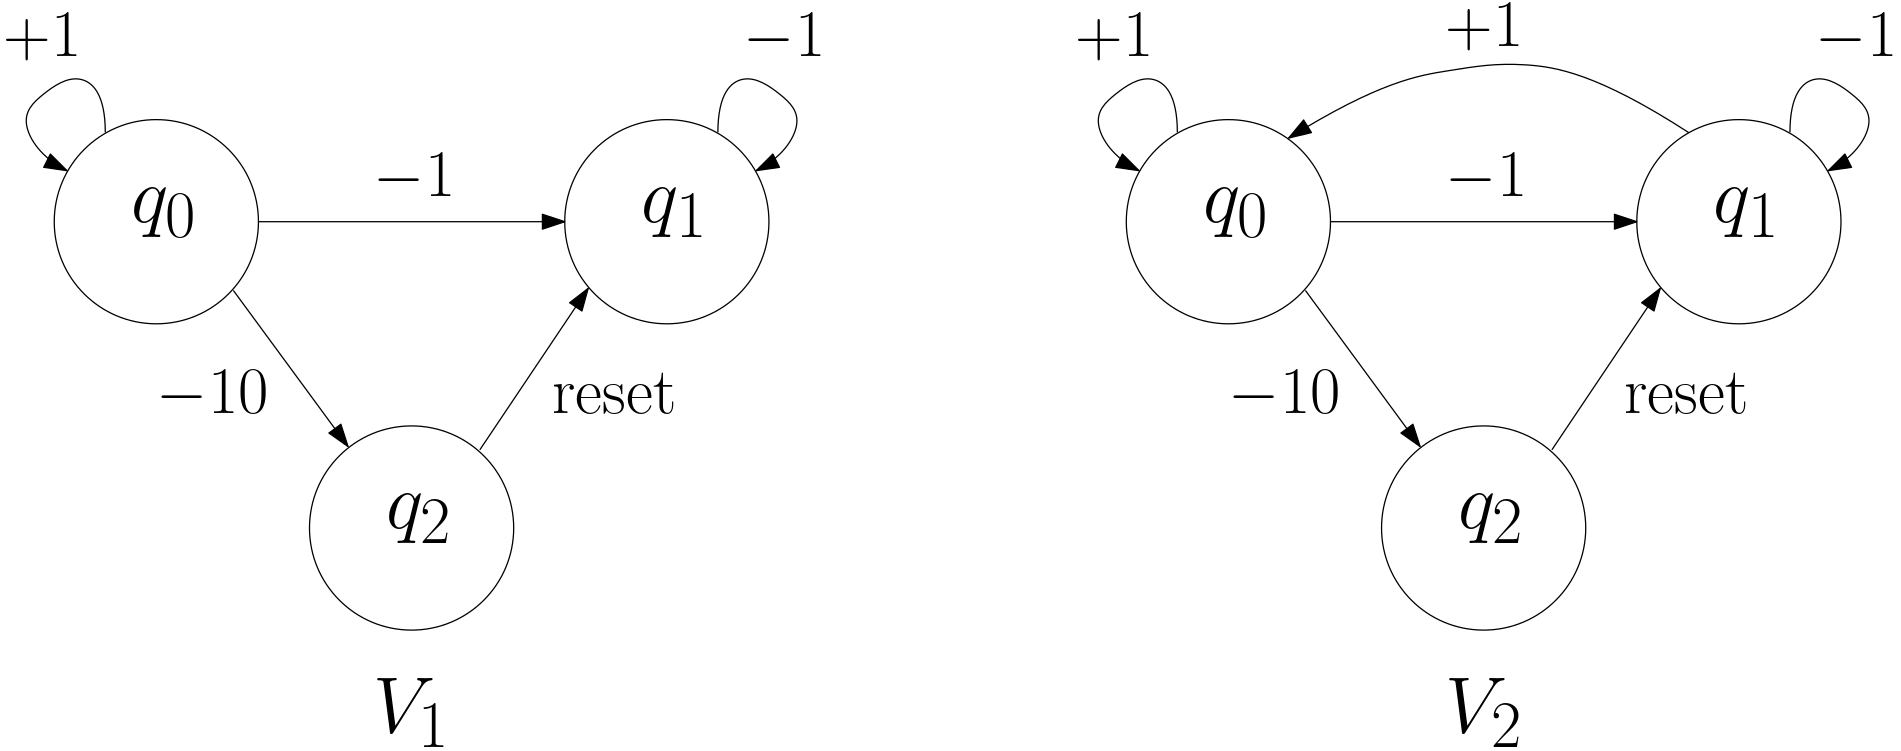
\includegraphics[width=0.75\textwidth]{FigureCD}
	\caption{Two reset-VASS with three control-states and one counter.}
					\label{r-V}
	\end{figure}
\end{center}

\begin{example}\label{Example}
{(\bf Reset-VASS example).}
Consider the 
 reset-VASS $V_1$ from Figure~\ref{r-V}.
Consider first $\Safe = \{q_0(n) \mid n \in \N\}$; In this case,  {resilience}, 
{$k$-resilience} and {bounded resilience} are not satisfied: there is no  way back from $q_2$ or $q_1$ to $q_0$. Consider now $\Safe = \{q_1(0)\} $; then {resilience} hold: it is possible to reach $q_1(0)$ from any state of $V_1$. However, {bounded resilience} does not hold, since, for all $n\in \N$, from $q_1(n)$, there is no path of length less than $n$ towards $q_1(0)$. Consider now the 
 reset-VASS $V_2$, which is $V_1$ plus an $+1$ transition from $q_1$ back to $q_0$. In $V_2$, {bounded resilience} hold, since $6$-resilience hold. 
Indeed, from any state with value of the counter bigger than $9$, it is possible to reach $q_2$ in two steps or less, then use the (unique) reset transition. From $q_1(n)$ or $q_0(n)$ with $n \in \{1, 2, 3, 4, 5, 6\}$ it is possible to reach $q_1(0)$ in $6$ steps or less. From 
$q_1(n)$ or $q_0(n)$ with $n \in \{7,8\}$ it is possible to reach $q_0(10)$ in $3$ steps or less, from which $q_1(0)$ is reachable in $2$ steps. 
\end{example}

% Hence we can see how adding transitions can 
% turn a system that is not bounded resilient into one that is. 
% \alain{à quoi sert cette remarque ?}




\section{Well-structured transition systems and VASS}\label{section definitions}



\noindent
 A {\em transition system} is a pair $\mathscr{S} = (S,\rightarrow )$ where $S$ is a set of 
 {\em states} and  
 $ {\rightarrow} \subseteq S \times S$ is a
 binary relation 
 on
 the set of states, denoted as the set of {\em transitions}. 
%
We write $s \rightarrow s'$ to denote $ (s,s') \in  {\rightarrow} $.
We write $\rightarrow^{k}$, $\rightarrow^{+}$, $\rightarrow^{=}$, $\rightarrow^{*}$
for the $k$-step iteration of $\rightarrow$, its transitive closure, its reflexive closure, its reflexive and transitive closure.
Let $X,Y \subseteq S$ and $k \in \mathbb{N}$; we denote $X \longrightarrow^{*} Y$ (resp. $X \longrightarrow^{\leq k} Y$) if from all states $x \in X$ there exists a path (resp. of length smaller than $k$) that reaches a state $y \in Y$.
\noindent
The set of {\em (immediate) successors} of a state $s \in S$ is defined as 
 $\post_{\mathscr{S}}(s) = \{ s' \in S \mid  ~ s \xrightarrow{} s'\}$. 
The set of {\em (immediate) predecessors} of a state $s \in S$ is defined as
 $\pred_{\mathscr{S}}(s) = \{ s' \in S \mid  ~ s' \xrightarrow{} s\}$. 
To simplify the notations, we write without ambiguity $\post_{\mathscr{S}}(D)$ by $\post(D)$ and  $\pred_{\mathscr{S}}(D)$ by  $\pred(D)$.
By iterating $\pred$ and $\post$ we obtain  
$\post^n(s) = \{ s' \in S \mid  ~ s \xrightarrow{}^n s'\}$
and
$\pred^n(s) = \{ s' \in S \mid  ~ s' \xrightarrow{}^n s\}$.
However, we are generally more interested in
$\post^{\leq n}(s) = \bigcup_{1 \leq i \leq n} \post^i(s)$, $\post^*(s)= \bigcup_{1 \leq i} \post^i(s)$
and
$\pred^{\leq n}(s) = \bigcup_{1 \leq i \leq n} \pred^i(s)$ and $\pred^*(s) = \bigcup_{1 \leq i} \pred^i(s)$. 
The {\em reachability problem} asks, given a transition system $\mathscr{S} = (S, \to)$, two states $s, t \in S$, whether $s \to^* t$. 

%


A {\em quasi-ordering} (a qo) is any reflexive and transitive relation $\leq$ over some set $X$ and we often write $(X,\leq)$. 
Given a quasi-ordering $(X,\leq)$, an {\em upward-closed set} is any set $U \subseteq X$ such that if $x \leq y$ and $x \in U$ then $y \in U $.
A {\em downward-closed set} is any set $D \subseteq X$ such that if $y \leq x$ and $x \in D$ then $y \in D $. 
It is an {\em ideal } if it is also {\em directed}, i.e. it is nonempty and for every $a,b \in D$, there exists $c \in D$ such that $a \leq c$ and $b \leq c$.
To any subset $A \subseteq X$, we may associate
its {\em upward-closure},
 $\mathop{\uparrow} A = \{x \in X \mid \exists a \in A ~ a \leq x\}$
 and its 
 {\em downward-closure},
 $\mathop{\downarrow} A = \{x \in X \mid \exists a \in A ~ x \leq a\}$. 
We abbreviate $\mathop{\uparrow} \{x\}$ (resp. $\mathop{\downarrow} \{x\}$)
as $\mathop{\uparrow} x$ (resp. $\mathop{\downarrow} x$).
%
A {\em basis} of an upward-closed set $U$ is a set $U_b$ such that $U = \mathop{\uparrow} U_b$; similarly, a {\em basis} of a downward-closed set $D$ is a set $D_b$ such that $D = \mathop{\downarrow} D_b$.


 A {\em well-quasi-ordering} (wqo) is any quasi-ordering $(X,\leq)$ such that, for any infinite sequence $x_0, x_1, x_2, ...$ in $X$, there exist indexes $i \leq j$ with $x_i \leq  x_j$. This property is equivalent to the \emph{finite decomposition} property : every upward-closed set $\emptyset \neq U \subseteq X$ admits a finite basis $B \subseteq X$ such that $U=\mathop{\uparrow} B$.
%
%
%
Wqo admits many other equivalent formulations like : a qo $(X,\leq)$ is a wqo iff $(X,\leq)$ is well founded (i.e. there is no infinite strictly decreasing sequence
of elements of $X$) and $(X,\leq)$ contains no infinite antichains (an antichain is a subset of mutually incomparable elements of $X$). See other equivalences in \cite{DBLP:phd/hal/Halfon18,schmitz:cel-00727025}. 
%
%
As an example, $(\N^d, \leq)$, the set of vectors of $d$ natural numbers (where $d$ is finite) with component-wise order is a wqo.\\
Quasi-orderings that have no 
infinite antichains
 enjoy a similar \emph{finite decomposition} property than wqo: every downward-closed subset $D \subseteq X$ can be decomposed into a \emph{finite} set of ideals $J_1, J_2, \ldots, J_n$ such that $D = J_1 \cup J_2 \cup \ldots \cup J_n$ See for example \cite{BFM-ic17}.
%
%
In what follows, a downward-closed set $D$ is represented by its finite set of ideals (or by the minimal elements of its upward-closed complement), and an upward-closed set $U$ is represented by its finite set of minimal elements. \\

\noindent
Let us now recall the (most general) definition of well-structured transition systems.
\begin{definition}[Definition 3.10, \cite{DBLP:journals/iandc/Finkel90}]
A {\em Well-Structured Transition System} (WSTS)  $\mathscr{S}=(S, \rightarrow, \leq)$
is a transition system $(S, \rightarrow)$
equipped with a wqo ${\leq} \subseteq S \times S$ such that   
the transition relation $ \rightarrow$ is (upward) compatible with $\leq$, i.e., for all 
$s_1, t_1 , s_2 \in S$
	with $s_1 \leq s_2$  and $s_1 \rightarrow t_1$, there exists 
	$t_2 \in S$ with 
	$t_1 \leq t_2$ and $s_2 \rightarrow^{*} t_2$.
\end{definition}

An (upward) compatible transition relation $ \rightarrow$ is \emph{reflexive} when the sequence $s_2 \rightarrow^{*} t_2$ is not empty: formally,
for all 
$s_1, t_1 , s_2 \in S$
	with $s_1 \leq s_2$  and $s_1 \rightarrow t_1$, there exists 
	$t_2 \in S$ with 
	$t_1 \leq t_2$ and $s_2 \rightarrow^{+} t_2$.
%
We say that a WSTS $\mathscr{S}$ has \emph{strong (upward) compatibility} when moreover for all 
$s_1, t_1 , s_2 \in S$
	with $s_1 \leq s_2$  and $s_1 \rightarrow t_1$, there exists 
	$t_2 \in S$ with 
	$t_1 \leq t_2$ and $s_2 \rightarrow t_2$.


Several families of formal models of processes  \cite{DBLP:journals/tcs/FinkelS01} give rise to WSTSs in a natural way with disfferent compatibilities, e.g. compatible counter machines like VASS with $d$ counters and $Q$ a finite set of control-states (and equivalently Petri nets) data Petri nets, reset/transfer VASS are WSTS with strong compatibility for the usual ordering $=\times \leq^d$ on the set of states $S=Q \times \N^d$.
Similarly, lossy channel systems with $d$ channels and $Q$ a finite set of control-states are WSTS (with a non-strong compatibility)
for the ordering $=\times \sqsubseteq^d$ (where $\sqsubseteq$ is the subword ordering on $\Sigma^*$) on $S= Q \times (\Sigma^*)^d$.\\
%%%%

But there is a more general class of (upward) compatible ordered transition systems than WSTS for which coverability is still decidable: recall that a Well Behaved Transition System (WBTS) \cite{DBLP:journals/lmcs/BlondinFM17} is an upward compatible ordered transition system $\mathscr{S}=(S, \rightarrow, \leq)$ where $(S,\leq)$ that contains no infinite antichains (but it can be not well founded). The class of WBTS is strictly larger than WSTS: for example, $\mathbb{Z}^d-$VASS under the lexicographical ordering are WBTS but not WSTS \cite{DBLP:journals/lmcs/BlondinFM17}. \\

By applying Proposition~4.3 from \cite{DBLP:journals/corr/abs-1208-4549}, we can reintroduce a straightforward definition of a specific proper subset of wqos that allow to construct coverability trees: 

\begin{definition}
A wqo $(X, \leq)$ is an \emph{$\omega^2$-wqo} if $(Ideals(X), \subseteq)$ forms a wqo.
\end{definition}

%Using Proposition~4.3 in \cite{DBLP:journals/corr/abs-1208-4549}, we recall a simple definition of a strict subclass of wqos that has a very nice property: a wqo $(X,\leq)$ is an $\omega^2$-wqo iff $(Ideals(X),\subseteq)$ is a wqo. 

Although there exists wqo that are not $\omega^2$-wqo (see the Rado ordering in \cite{DBLP:journals/ipl/Jancar99}), all naturally occurring wqos are $\omega^2$-wqo, perhaps to the notable exception of finite graphs well-quasi-ordered by the graph minor relation. %			which are wqo but not known to be $\omega^2$-wqo. 
The class of $\omega^2$-wqo is robust because every datatype in the following list - natural number, finite set, finite product, finite sum, finite disjoint sum, finite words, finite multisets and finite trees - is an $\omega^2$-wqo (Proposition~4.5 in \cite{DBLP:journals/corr/abs-1208-4549}). Now we are able to define $\omega^2$-WSTS:

\begin{definition}(Finkel and Goubault-Larrecq \cite{DBLP:journals/corr/abs-1208-4549})
A WSTS  $\mathscr{S}=(S, \rightarrow, \leq)$
is an $\omega^2$-WSTS if $(S, \leq)$ is an $\omega^2$-wqo.
\end{definition}
Since almost of usual wqo are $\omega^2$-wqo, all naturally occurring WSTS are in fact $\omega^2$-WSTS: for example, reset/transfer VASS are $\omega^2$-WSTS.\\
%%%%%%

Let us recall that the \emph{completion}  \cite{BFM-ic17} of a WSTS $\mathscr{S}=(S,\rightarrow, \leq)$ is the associated ordered transition system $\hat{\mathscr{S}}=(Ideals(S),\rightarrow, \subseteq)$ where $Ideals(S)$ is the set of ideals of $S$ and $I \rightarrow J$ if $J$ belongs to the finite ideal decomposition of $\mathop{\downarrow} \post_{\mathscr{S}}(I)$. The completion is always \emph{finitely branching} but it is not necessarly a WSTS since $\subseteq$ is not necessarly a wqo. It is proved in  \cite{BFM-ic17} that $\hat{\mathscr{S}}$ is WSTS iff $\mathscr{S}=(S,\rightarrow, \leq)$ is $\omega^2$-WSTS. \\

Another type of WSTS exists that enjoys downward compatibility.
%
%		Finkel and Schnoebelen, 
%
\begin{definition}[Definition 5.1, \cite{DBLP:journals/tcs/FinkelS01}]
A {\em downward (compatible) well-structured transition system} (downward-WSTS)  $\mathscr{S}=(S, \rightarrow, \leq)$
is a transition system $(S, \rightarrow)$
equipped with a wqo ${\leq} \subseteq S \times S$ such that   
the transition relation $ \rightarrow$ is downward compatible with $\leq$, i.e., for all 
$s_1, t_1 , s_2 \in S$
	with $s_2 \leq s_1$  and $s_1 \rightarrow t_1$, there exists 
	$t_2 \in S$ with 
	$t_2 \leq t_1$ and $s_2 \rightarrow^{*} t_2$.
\end{definition}

There are fewer downward-WSTS than WSTS, but we can still mention FIFO automata with insertion errors and Basic Process Algebra (BPA).

Let us reformulate the downward compatibility property.

\begin{lemma}\label{downward compatible}
For an ordered transition system $\mathscr{S}=(S, \rightarrow, \leq)$ (not necessarly a WSTS), the two following properties are equivalent: (1) $\mathscr{S}=(S, \rightarrow, \leq)$ is downward compatible ; (2) for every downward-closed set $D \subseteq S$, the set $\pred_{\mathscr{S}}^*(D)$ is downward-closed.
\end{lemma}

\begin{proof}
Let us prove $1 \implies 2$. 
Let $D$ be a downward-closed subset of $S$
and let $x \in \mathop{\downarrow} \pred^*(D)$.
By downward closure, there exists
$y \in \pred^*(D)$ 
such that $x \leq y$.
By definition of $\pred^*(D)$, there exists 
$d \in D$ such that: (1) either $y=d$ and then $x \in D \subseteq \pred^*(D)$ or (2) there exist $m\geq 0$ and $(a_i)_{0 \leq i \leq m+1} \in S^{m+2}$ such that
$y = a_0 \to a_1 \to a_2 \to \cdots \to a_m \to a_{m+1} = d$.
%
By downward compatibility $a_0 \to a_1$
implies that there exists $a'_1 \in S$ such that $a'_1 \leq a_1$ and
$x \to^* a'_1$.
More generally $a_i \to a_{i+1}$ and
$a'_i\leq a_i$ implies the existence of $a'_{i+1} \in S$ with $a'_{i+1} \leq a_{i+1}$ and
$a'_i \to^* a'_{i+1}$,
and, by induction,
 $x \to^* a'_1 \to^* \cdots \to^* a'_{m} \to^* a'_{m+1} = d'$
with $d' \leq d$.
Since
$d'$ 
belongs to $D$ by downward closure of $D$, $x \in \pred^*(D)$ and then $\mathop{\downarrow}\pred^*(D) \subseteq \pred^*(D)$. Since $\pred^*(D) \subseteq \mathop{\downarrow} \pred^*(D)$ always hold, we deduce that $\pred^*(D)=\mathop{\downarrow}\pred^*(D)$ is downward-closed.

Let us prove $2 \implies 1$. Let $s_1, t_1 , s_2 \in S$ with $s_2 \leq s_1$  and $s_1 \rightarrow t_1$, Since $s_1 \rightarrow t_1$ we deduce that $s_1 \in \pred^*(\mathop{\downarrow} t_1)$, and since $s_2 \leq s_1$ and $\pred^*(\mathop{\downarrow} t_1)$ is downward-closed, we also have $s_2 \in \pred^*(\mathop{\downarrow} t_1)$. This means that there exists $t_2 \leq t_1$ such that 
$s_2 \rightarrow^{*} t_2$. Hence, we proved that $\mathscr{S}$ is downward compatible.
\qed
\end{proof}

%A WSTS $\mathscr{S}=(S,\rightarrow,\leq)$ is {\em completion-$\post$-effective} if
%it is $\post$-effective, and there exists an algorithm $M_\downarrow$ that computes 
% $\downarrow s$, on input $s \in S$, and some algorithm $M_{\mathop{\uparrow}^C}$ that computes the ideal decomposition of $S \setminus \mathop{\uparrow} \{ s_1, s_2, \ldots, s_m\}$, on input
% $s_1, s_2, \ldots, s_m \in S$.


To obtain decidability results, we must introduce some notions of \emph{effectiveness}. We use a mixture of the notions defined both by Blondin and al. in \cite{DBLP:journals/lmcs/BlondinFM17}) and by Halfon in \cite{DBLP:phd/hal/Halfon18}.
%			 that will be essential for solving various resilience problems in different models of WSTS. 
First, to simplify, we suppose that all classes of considered ordered transition systems $\mathscr{S}=(S, \rightarrow, \leq)$ satisfy the five following properties:
\begin{enumerate}
\item there exists an algorithm that decides whether $s \rightarrow t$ is true or not, for any states $s,t \in S$,
%
\item there is a computational representation for $S$ for which membership in $S$ is decidable,
%
%			We also suppose that all considered wqos $(S,\leq)$ satisfy the three following conditions : 
\item $\leq$ is decidable,
\item there is a computational representation for $Ideals(S)$ for which membership in $Ideals(S)$ is decidable, and
\item  inclusion of ideals is decidable. 
\end{enumerate}
%
Blondin and al. showed (Lemma 4.3 in \cite{DBLP:journals/lmcs/BlondinFM17}) that under the previous hypotheses, one are able to enumerate \emph{downward-closed sets} (by their finite decomposition in ideals), to decide inclusion between downward-closed sets and to decide if a state belongs to a given finite set of ideals. But the five properties are not sufficient to compute the complementary and the intersection of downward-closed sets.
%
Halfon introduced \emph{ideally-effective wqo} as wqo that essentially allow to compute representations of (principal) ideals $\mathop{\downarrow} s$, of the complementary of an ideal, of the complementary of filters (a filter is a set $\mathop{\uparrow} s$ for $s \in S$) and to compute representations of finite intersections of filters and finite intersections of ideals. Most well-known wqo are ideally-effective . \cite{DBLP:phd/hal/Halfon18}.
%	 (hence of downward-closed sets).

%
Starting now, we assume that all considered WBTS $\mathscr{S}=(S, \rightarrow, \leq)$ satisfy the five previous properties and that the wqo $\leq$ is ideally-effective. We refer to such WBTS as \emph{effective}.

In order to construct algorithms, we also require effective hypotheses about the computations of certain sets of predecessors and successors. More precisely, we say that an ordered transition system $\mathscr{S}=(S, \rightarrow, \leq)$ is 
\begin{enumerate}
%\item {\em effective} if there exists a pair of algorithms
%($M_\rightarrow$, $M_\leq$) operating on $\N \times \N$ such that
%$ M_\rightarrow$ computes the transition relation “$\rightarrow$” and 
%$M_\leq$ the ordering relation “$\leq$”.
%
\item {\em $\post$-effective} if $\mathscr{S}$ is effective, and if there
exists an algorithm that computes $|\post(s)| \in \N \cup \{\infty\}$ 
on input $s \in S$.
%
%\item {\em ideally-effective} \cite{BFM-ic17} if the function mapping the encoding of a state $s$
%to the encoding of the ideal $\downarrow s$ is computable.
%
\item {\em $\post$-ideal-effective} if $\mathscr{S}$ is effective and there exists an algorithm accepting
any ideal $I \in Ideals(S)$ and returning $\mathop{\downarrow} \post(I)$, expressed as a finite union of (maximal) ideals.
%\item {\em completion-$\post$-effective} if its completion $\hat{\mathscr{S}}=(Ideals(S),\rightarrow, \subseteq)$ is $\post$-effective, i.e., that $\downarrow \post(I)$ is computable, expressed as a finite union of ideals, for all $I \in Ideals(S)$.
%
\item {\em $\pred$-basis-effective} \cite{DBLP:journals/tcs/FinkelS01,DBLP:journals/iandc/AbdullaCJT00} if $\mathscr{S}$ is effective and there exists an algorithm accepting
any state $s \in S$ and returning a finite basis of $\mathop{\uparrow} \pred(\mathop{\uparrow} s)$.
%
%and there exist an algorithm $M_\downarrow$ that computes 
% $\downarrow s$, on input $s \in S$, and some algorithm $M_{\mathop{\uparrow}^C}$ that computes the ideal decomposition of $S \setminus \mathop{\uparrow} \{ s_1, s_2, \ldots, s_m\}$, on input
% $s_1, s_2, \ldots, s_m \in S$.
%
\item {\em $\post^*$-basis-effective} \cite{DBLP:conf/gg/Ozkan22,DBLP:journals/corr/abs-2108-00889} if $\mathscr{S}$ is effective and there exists an algorithm accepting
any state $s \in S$ and returning a finite basis of $\mathop{\uparrow} \post^*(s)$.
%
\item {\em $\pred^*$-basis-effective} if $\mathscr{S}$ is effective and there exists an algorithm accepting
any ideal $I \in Ideals(S)$ and returning a finite basis of $\mathop{\downarrow} \pred^*(I)$.
\end{enumerate}

Counter machines are effective but don't enjoy any other effectivities among the list of five.
Reset VASS (hence VASS) and (front) lossy fifo automata are $\post$-effective, $\post$-ideal-effective, and $\pred$-basis-effective. There exist $\post$-effective WSTS that are not $\post$-ideal-effective (Proposition~35 in \cite{BFM-ic17}); there exist $\post$-ideal-effective WSTS that are not $\post$-effective (Proposition~36 in \cite{BFM-ic17}).There also exist WSTS that are not $\pred$-basis-effective (Proposition~45 in \cite{BFM-ic17}).
Reset VASS are not $\post^*$-basis-effective since $\post^*$-basis-effectiveness allows to compute the finite set of the set of minimal reachable states, hence it would allow to decide the zero-reachability problem that is undecidable for reset-VASS. However, VASS are $\post^*$-basis-effective \cite{DBLP:journals/corr/abs-2108-00889} and LCS (with $d$ fifo channels) are also $\post^*$-basis-effective because we have $(q,w_1,w_2,...,w_d) \in \mathop{\uparrow} \post^*(q_0,u_1,u_2,...,u_d)$ iff $(q,\epsilon,...,\epsilon)  \in \mathop{\uparrow} \post^*(q_0,u_1,u_2,...,u_d)$ iff $(q,\epsilon,...,\epsilon)$ is reachable from $(q_0,u_1,u_2,...,u_d)$ that is decidable in LCS.
%
Reset-VASS are not $\pred^*$-basis-effective because computing a finite basis of $\mathop{\downarrow} \pred^*(q,0,...,0)$ would allow to decide whether $(q,0,...,0)$ is reachable that is undecidable for reset-VASS.
By using the decidability of reachability and Theorem 3.11 in \cite{DBLP:journals/acta/ValkJ85}, we may prove that VASS are $\pred^*$-basis-effective. A more complete study of these properties will be done in the long version of this paper.




%Most of usual WSTS are $\post$-effective and ideally-effective.

% \alain{le rappel ci-dessous est-il entièrement utile ? Je pense qu'on peut l'enlever, et toi ?}
% Now, we may recall a simple condition that insures that a finite basis of $\pred^*(\mathop{\uparrow} s )$ is computable for every $s \in S$.
% We will use the following property: if $\mathscr{S}$ is a WSTS with strong compatibility and $U \subseteq S$ is upward-closed, then $\pred(U )$, $\pred^k(U )$ with $k\geq0$, and $\pred^*(U )$ are all upward-closed \cite{DBLP:journals/tcs/FinkelS01}.
% For a WSTS $\mathscr{S}=(S, \rightarrow, \leq)$ and an upward-closed set $U  \subseteq S$, let us study the convergence of the sequence defined by $U_0=U$ and $U_k= U_{k-1} \cup \pred(U_{k-1})$ for $k \geq 1$. When $\mathscr{S}$ has strong compatibility, the sets $U_k$ are upward-closed and $U_k \subseteq U_{k+1}$ so we know that the sequence $(U_k)_k$ converges. Let us define the \emph{index} of convergence of the sequence $U_k$ as the smallest $k_0$ s.t. $U_k = U_{k_0}$ for all $k \geq k_0$. We may compute $k_0$ and we then have:  $\pred^*(U) = U_{k_0}$. When $\mathscr{S}$ have upward-compatibility but not strong compatibility, we can similarly compute $\pred^*(U)$ by studying the sequence $(\mathop{\uparrow} U_k)_k$ instead.

Recall the \emph{coverability problem} for ordered transition systems.

\problemx{Coverability problem}
{An ordered transition system $\mathscr{S}=(S,\rightarrow, \leq)$ and two states $s_0,s \in S$.}
{ $s_0 \in \pred^*(\mathop{\uparrow} s )$ ? \newline}

%An equivalent formulation is : Does there exist $t \in S$ such that $s_0 \longrightarrow^{*} t$ and $s \leq t$ ?
With the $\pred$-basis-effective hypothesis, we obtain:
%
%			(Finkel and Schnoebelen, Abdulla and al., 
%
\begin{theorem}[Theorem 3.6, \cite{DBLP:journals/tcs/FinkelS01}, Theorem 4.1, \cite{DBLP:journals/iandc/AbdullaCJT00}]
 A finite basis of $ \pred^*(U)$ is computable for any $\pred$-basis-effective WSTS $\mathscr{S}=(S, \rightarrow, \leq)$ and any upward-closed set $U \subseteq S$ given with its finite basis $B_U$. Hence coverability is decidable.
\end{theorem}

With the $\post$-ideal-effective hypothesis, we obtain the decidability of coverability for WBTS (without the $\pred$-basis-effective hypothesis).
%
%		(Blondin and al., 
%
\begin{theorem}[Corollaire 4.4, ~\cite{DBLP:journals/lmcs/BlondinFM17}]
Coverability is decidable for any $\post$-ideal-effective WBTS.
\end{theorem}

Downward-WSTS enjoy a powerfull property.
%
%		Finkel and Schnoebelen, 
%
\begin{theorem}[Proposition 5.4, \cite{DBLP:journals/tcs/FinkelS01}]
Finitely branching downward-WSTS with reflexive compatibility and $\post$-effective are $\post^*$-basis-effective.
\end{theorem}
%
%Coverability is  decidable for a class of WSTS without the effective $\pred$-basis hypothesis.
%
%\begin{theorem} \cite{BFM-ic17}
%Coverability is decidable for ideally-effective WSTS.
%\end{theorem}

Let us recall the  definition of vector addition system with (control-)states. 
 \begin{definition} 
A {\em vector addition system with (control-)states (VASS)} in dimension $d$ ($d$-VASS for short) is a finite $\mathds{Z}^d$-labeled directed graph $V = (Q,T)$, where $Q$ is the set of {\em control-states}, and $T \subseteq Q \times \mathds{Z}^d \times Q$ is the set of {\em control-transitions}. 
 \end{definition} 
%
Subsetquently, $Q \times \N^d$ is the set of states of the transition system associated with a $d$-VASS $V$.
For all states $p(\textbf{u}), q(\textbf{v}) \in Q \times \N^d$ and for every control-transition $t = (p, \textbf{z}, q)$, we write $p(\textbf{u}) \xrightarrow{t} q(\textbf{v})$ whenever $\textbf{v} = \textbf{u} + \textbf{z} \geq \textbf{0}$.
%
When in the context of a $d$-VASS, we denote $0^d$ by $\textbf{0}$.

A {\em vector addition system (VAS)} in dimension $d$ ($d$-VAS for short) is a $d$-VASS where the set of control-states is a singleton; hence one only needs $T$.\\

VASS can be extended with resets.

\begin{definition}
A {\em reset-VASS} in dimension $d$ 
 is a finite 
labeled directed graph $V = (Q,T)$, where $Q$ is the set of {\em control-states}, 
$T \subseteq Q \times Op \times Q$
is the set of {\em control-transitions}, and $Op = \{ add(\textbf{z}) \mid \textbf{z} \in \mathds{Z}^d\} \cup 
		\{ reset(i) \mid i \in \{1,\ldots,d\} \}$.
\end{definition}

%Again $Q \times \N^d$
% is the set of states of $V$.
For every states $p(\textbf{u}), q(\textbf{v}) \in Q \times \N^d$ and every control-transition $t$ we write
$p(\textbf{u}) \xrightarrow{t} q(\textbf{v})$ when 
\begin{samepage}\begin{itemize}
\item  $t = (q,add(\textbf{z}),q') \in T$
and $\textbf{u}+\textbf{z} = \textbf{v} \geq 0$,
\item $t = (q,reset(i),q') \in T$ 
and
$\textbf{v}[i] = 0$, and $\textbf{v}[i'] = \textbf{u}[i']$ for all $i' \in \{1,\ldots, d\} \setminus i$.
\end{itemize} \end{samepage}

As an example, let us remark that $(\N^d,\leq)$ is an ideally-effective wqo.

 \begin{center}
	\begin{figure}
	\hspace{2.3cm}
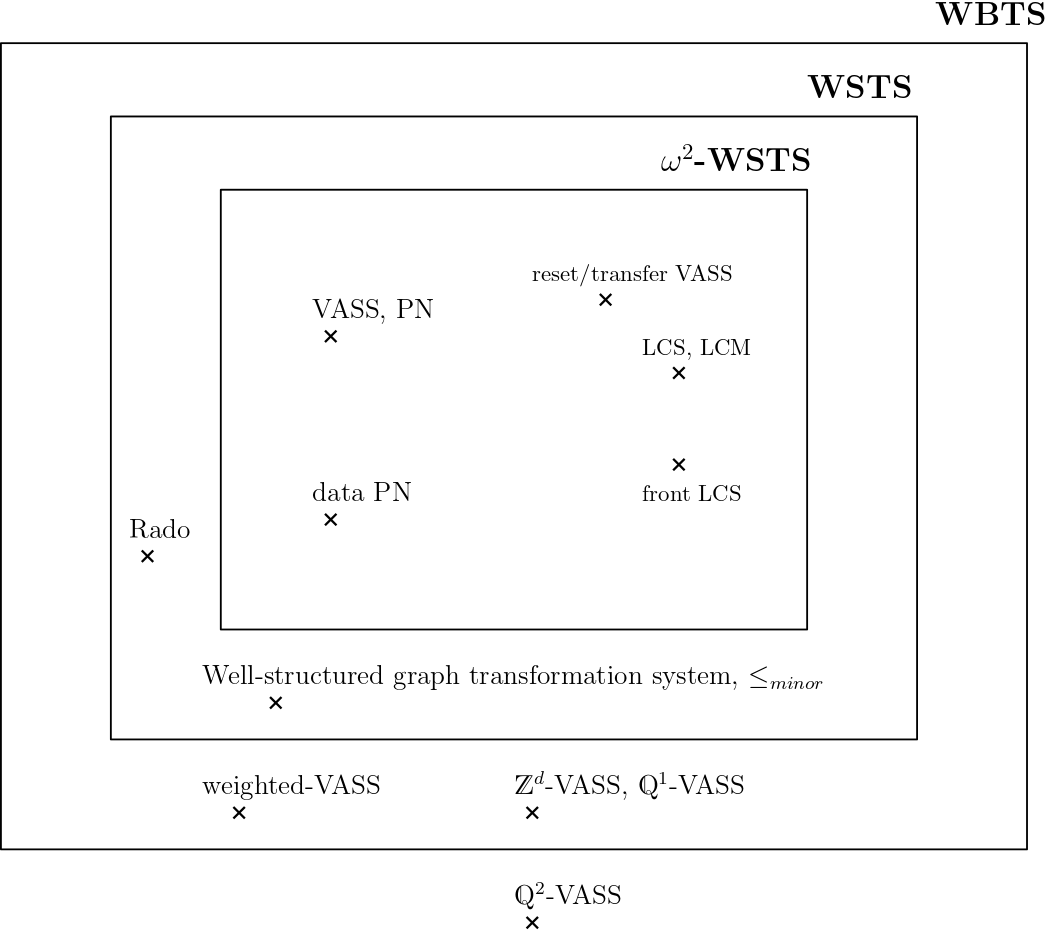
\includegraphics[width=0.60\textwidth]{WSTS_taxonomy}
	\caption{A taxonomy of WSTS and variants.}
	\end{figure}
\end{center}


\section{Resilience for WSTS}



In a (not necessarly ordered) transition system $\mathscr{S}=(S,\rightarrow)$, we consider a subset of states $\Safe \subseteq S$, and its complement, $\Bad$.
The \emph{resilience problem} (resp. the \emph{$k$-resilience problem}) for $(\mathscr{S},\Safe)$ is to decide whether from \emph{any} state in 
$S$, \emph{there exists} a path (resp. a path of length smaller than or equal to $k$) that reaches a state in $\Safe$. Resilience is then akin to the Home-Space problem (defined in the introduction) for the set $\Safe$. Resilience can also be viewed as a generalizeation
 of coverability, as
it asks whether for \emph{every} element of $\Bad$ it is possible to cover an element of the basis of $\Safe$.
We use the notation 
$S \longrightarrow^{*} \Safe$ (resp. $S \longrightarrow^{\leq k} \Safe$)
 for 
$\forall x \in S, \exists y \in \Safe$ 
 such that $x \longrightarrow^{*} y$ 
  (resp.  $\forall x \in S, \exists y \in \Safe$ such that $x \longrightarrow^{\leq k} y$).
  In our framework, $\Safe \subseteq S$  is possibly infinite but  must admit a computable finite representation : for example, downward-closed sets and upward-closed sets in wqos and semilinear sets in $\mathbb{N}^d$ have finite representations. 





Let us formalize three resilience problems.


\problemx{Resilience (RP)}
{A transition system $\mathscr{S}=(S,\rightarrow)$ and a set $\Safe \subseteq S$.}
{$S \longrightarrow^{*} \Safe$ ?\newline}



\problemx{$k$-resilience (kRP)}
{A transition system $\mathscr{S}=(S,\rightarrow), k \in \mathbb{N}$ and a set $\Safe \subseteq S$.}
{$S \longrightarrow^{\leq k} \Safe$ ?\newline}

\problemx{Bounded resilience (BRP)}
{A transition system $\mathscr{S}=(S,\rightarrow)$ and a set $\Safe \subseteq S$.}
{$\exists k \geq 0$ such that {$S \longrightarrow^{\leq k} \Safe$ ?\newline}}




These three resilience problems are decidable for finite transition systems but undecidable for (general) infinite-state transition systems. So we restrict our framework to the class of infinite-state WSTS. Since most of decidable properties in WSTS rely on the computation of upward or downward-closed sets \cite{DBLP:journals/iandc/AbdullaCJT00,DBLP:journals/tcs/FinkelS01}, we consider upward-closed or downward-closed sets $\Safe$% and $\Bad$
. Since $\Safe \subseteq \pred^*(\Safe)$, one only needs to decide whether 
the complement of $\Safe$ is in $\pred^*(\Safe)$. From now on, we use $\Bad$ to denote the complement of $\Safe$.\\
%In   	 \cite{DBLP:journals/corr/abs-2108-00889}, the authors considered that $\Safe$ is upward-closed.  \\

Surprisingly, the general undecidability statement regarding resilience had neither been known nor proven.
We show that the resilience problem is undecidable for $\omega^2$-WSTS with strong compatibility. 
%
% \alain{pourquoi n'a-t-on pas prouvé la même chose pour la BR et la k-R ?: où est la difficulté ?}
\begin{proposition}\label{indec WSTS}
{\sc Resilience} for $\post$-effective $\omega^2$-WSTS with strong compatibility, for upward closed sets $\Safe$ is undecidable.
\end{proposition}
% \alain{peut-on ajouter des hypothèses d'effectivity ? peut-on montrer que l'exemple n'est pas pred effectif ? l'exemple est-il  ideal-effective (oui pour les propriétes 1 et 2 mais pas 3 car ça permettrait de décider l'arrêt ?)? on voit que l'exemple n'est pas completion-$\post$-effective vu le theoreme qui suit}
\begin{proof}
Indeed, consider the family $\{ f_j: \N^2 \to \N^2\}$ of 
increasing recursive functions from \cite{FMP-ic04} defined as

$ f_j(n,k) = \begin{dcases*} (n,0) & \text{ if } k=0 \text{ and } TM$_j$ \text{ runs for more than } n \text{ steps} \\
		(n,n+k) &\text{ otherwise,} \end{dcases*} $
		
	\noindent	
	where TM$_j$ is the $j$-th Turing machine (in a classical enumeration)
	which moreover begins
by writing the integer $j$ on its tape,	
	and consider additionnally the function $g : \N^2 \to \N^2$ defined by $g(n,k) = (n+1,k)$. 
	The
	transition system 
	$S_j = (\N^2, \{f_j, g\}, \leq)$ 
	is a $\post$-effective $\omega^2$-WSTS with strong compatibility
	and
	has the property that
	it is
	$\mathop{\uparrow} (1,1)$-resilient
	iff TM$_j$ halts on input $j$,
	since $(1,1)$ is coverable from $(0,0)$
	iff TM$_j$ halts on input $j$. 
	Hence there is no Turing machine which correctly determines 
	resilience and halts whenever its input is a
	WSTS.
Hence resilience for $\omega^2$-WSTS with strong compatibility is undecidable.\qed
\end{proof}
 Let us remark that the transition system 
	$S_j = (\N^2, \{f_j, g\}, \leq)$ in the previous proof is not $\post$-ideal-effective
	nor $\pred$-basis-effective.
  
  
\mathieu{Reviewer 1: the example at the bottom of \textbf{ page~\pageref{indec WSTS}}, even if it is a WSTS, is a very particular case [...] wonder if classes containing such  systems are interesting per se. }


In the case of $\pred$-basis-effective upward compatible WSTS, {\sc Resilience} is undecidable when $\Safe = \mathop{\downarrow} \Safe$.


\begin{proposition}\label{indec WSTS with dcs}
{\sc Resilience} is undecidable for reset-VASS, hence it is also undecidable for $\pred$-basis-effective $\omega^2$-WSTS with strong compatibility and with 
$\Safe=\mathop{\downarrow} \Safe$.
\end{proposition}


\begin{proof}
First, note that {\sc Resilience} is undecidable for a Minsky machine $M$ with at least $3$ counters when
$\Safe = \mathop{\downarrow} \Safe$,
since it is possible to guarantee that state $q_f(0,0,0)$ is the only element 
% of $Q_{M} \times \mathop{\downarrow} (1,1,0)$
potentially reachable from 
$\Bad = Q_{M} \times \mathop{\uparrow} (0,0,1)$ that is not already inside $\Bad$.
Now, executions of Minsky machines can be simulated by reset-VASS~\cite{araki1976PN,dufourd1998reset} in such a way that any sequence 
% from  a state $p({\bf u})$
% to
reaching
 a state 
%
$ q({\bf 0})$ corresponds to one that reaches 
$q_f(0,0,0)$
 in the Minsky machine and vice versa.
 Moreover, the reset-VASS is able to emulate zero tests on the counters, hence it is able to guarrantee that $ q({\bf 0})$ is its only $\Safe$ state reachable from a $\Bad$ state as well.
 By combining both constructions, which can be seen in more details in Appendix~\ref{minsk},
 we obtain that 
 {\sc Resilience} is undecidable for reset-VASS when $\Safe = \downarrow \Safe$, and hence for  $\post$-effective, $\pred$-basis-effective, 
$\omega^2$-WSTS with strong compatibility as well.
%\mathieu{preuve résumé / concise à écrire}
\iffalse
\alain{preuve pas claire, à réécrire}
% \alain{les reset-VASS sont-ils effective $\post^*$-basis ?}
% \mathieu{non, sinon on aurait décidabilité pour la state résilience}
%This stems from the fact that it is undecidable for Minsky machines with more than one counter,
%which can be simulated by WSTS.
First, let us show that {\sc Resilience} is undecidable for Minsky machine with at least $3$ counters.
%	This is due to the undecidability of $2$-counter Minsky machine termination~\cite{Min61,Min67}.
From a $2$-counter Minsky machine $M$ with final control-state $q_f \in Q_M$, one can construct a $3$-counter Minsky machine $M'$ with final control-state $q_f' \in Q_{M'}$
such that machine $M$ terminates for all inputs iff machine $M'$ can reach $q_f'(0,0,0)$ from any input in $Q_{M'} \times \mathop{\uparrow} (0,0,1)$. 
%			with at least $1$ on its third counter. 
We build $M'$ to simulate $M$ until it reaches $q_f$, then decrease the first two counters until they reach $0$, then, and only then, finally decrease the third counter until it reaches $0$.
Remark that in the construction, from any input in $Q_{M'} \times \mathop{\uparrow}(0,0,1)$, it is not possible to reach an element in $Q_{M'} \times \{ (1,0,0), (0,1,0),(1,1,0)\}$.
Based on this construction, the problem of deciding whether the downward-closed set $Q_{M'} \times \mathop{\downarrow} (1,1,0)$ is reachable in the $3$-counter Minsky machine $M'$
% \alain{review 3: - p. 10: why not choose $\mathop{\downarrow}{(0,0,0)}$ instead of $\mathop{\downarrow}{(1,1,0)}$?}
from any input in $Q_{M'} \times \mathop{\uparrow}(0,0,1)$ is equivalent to the termination of machine $M$, that is undecidable ~\cite{Min61}. 
Hence {\sc Resilience} is undecidable for Minsky machines.

% \alain{écrire qqchose ici}
Now, executions of Minsky machines can be simulated by reset-VASS~\cite{araki1976PN,dufourd1998reset}. 
% \alain{\cite{araki1976PN} simule-t-il les Minsky machines et comment ?}
%Reset-VASS extend the basic VASS model with special “reset
%transitions” that set to $0$ some coordinates in the vector. 
%			Let us recall their definition here.
%      	it is well known that reset-VASS are WSTS~\cite{dufourd1998reset}.
The simulation operates by building a reset-VASS in which
there exists
 a sequence from 
an initial state %$(s,x_1 \ldots x_n)$
to
a state $ q(0,  \ldots 0)$ if and only if
there exists
a sequence
 in the Minsky machine
 from a corresponding initial state
 to
 the state $q_f(0,0,0)$
  (from Theorem~$5$ in \cite{araki1976PN}).
Hence $Q_{M'} \times \mathop{\downarrow} (1,1,0)$-resilience hold in the Minsky machine $M'$ iff 
resilience hold in the reset-VASS simulating $M'$.
Since reset-VASS can simulate executions of a Minsky machine, {\sc Resilience} is undecidable for reset-VASS and hence for  $\pred$-basis-effective, 
$\omega^2$-WSTS with strong compatibility as well.
%\alain{déjà dit avant en mieux omega2 et strong comp et $\post$-effective mais reset-VASS apportent effective $\pred$-basis et ideally-effective....}
\fi
\qed \end{proof}


\subsection{Case: $\Safe=\mathop{\uparrow} \Safe$.}\label{safe-up}

We start with the case $\Safe=\mathop{\uparrow} \Safe$, hence $\Bad=\mathop{\downarrow} \Bad$.
Since Resilience is undecidable for  $\omega^2$-WSTS with strong compatibility (Theorem \ref{indec WSTS}), we still consider WSTS, and even WBTS, with strong compatibility but by strengthening the assumptions of effectiveness (we now consider the $\post$-ideal-effective hypothesis) and we demonstrate that the three resilience problems are now decidable.




%
\begin{theorem}\label{down-up}
Let $\mathscr{S}=(S,\rightarrow, \leq)$ be a $\post$-ideal-effective WBTS with strong compatibility and a set $\Safe = \mathop{\uparrow} \Safe$.
{\sc Resilience}, {\sc Bounded resilience} 
and {\sc $k$-resilience} are decidable.
\end{theorem}

%\alain{a-t-on le même rsultat pour les WSTS avec pred* calculable ? J'ai enlevé l'hypothèse omega2 car j'ai l'impression qu'elle n'est pas utile...à vérifier}

\begin{proof}
Let us first recall two results in \cite{BFM-ic17} that are stated for WSTS but are also true for WBTS since the proofs rely only on compatibility and not on the property of wqo. Proposition 30 establishes a strong relation between the runs of a WSTS $\mathscr{S}=(S,\rightarrow, \leq)$ and the runs of its completion $\hat{\mathscr{S}}$. It states that if $x \xrightarrow{k} y$ in $\mathscr{S}$ then for every ideal $I \supseteq \mathop{\downarrow} x$, there exists an ideal $J \supseteq \mathop{\downarrow} y$ such that $I \xrightarrow{k} J$ in $\hat{\mathscr{S}}$. Proposition 29 establishes that if $I \xrightarrow{k} J$ in $\hat{\mathscr{S}}$ then for every $y \in J$, there exists $x \in I$ and $y' \geq y$ such that $x \xrightarrow{k'} y'$ in $\mathscr{S}$. Moreover, if $\mathscr{S}$ has transitive compatibility then $k’ \geq k$; if $\mathscr{S}$ has strong compatibility then $k’ = k$.
%

Let  $\{s_1,s_2,...,s_m\}$ be the (unique) minimal basis of $\Safe$ and  $\{J_1, J_2,...,J_n\}$ be the ideal decomposition of $\Bad$.
The resilience problem can be reduced to the following infinite number of instances of the coverability problem in $\mathscr{S}$: for all $x \in \Bad$ does there exist an $j$ such that $s_j$ is coverable from $x$. Let us show how this infinite set of coverability questions can be reduced to a \emph{finite} set of coverability questions in the completion $\hat{\mathscr{S}}=(Ideals(S),\rightarrow, \subseteq)$ of $\mathscr{S}=(S,\rightarrow, \leq)$. 


Let us prove that $s_j$ is coverable from $x$ in $\mathscr{S}$ if and only if $\mathop{\downarrow} s_j$ is coverable (for inclusion) from $\mathop{\downarrow} x$ in $\hat{\mathscr{S}}$.
%
Suppose that $s_j$ is coverable from $x$ then there exists a run $x \xrightarrow{k} y \geq s_j$. From Proposition~30, there exist an ideal $J$ and a run $\mathop{\downarrow} x \xrightarrow{k} J$ where $J \supseteq \mathop{\downarrow} y \supseteq \mathop{\downarrow} s_j$ in $\hat{\mathscr{S}}$, hence $\mathop{\downarrow} s_j$ is covered from $\mathop{\downarrow} x$.
Conversely, if $I \xrightarrow{k} J$ in $\hat{\mathscr{S}}$ with $\mathop{\downarrow} s_j \subseteq J$ then 
%	for every $y \in J$, 
there exists $x \in I$ and $y' \geq s_j$ such that $x \xrightarrow{k} y'  \geq s_j$ in $\mathscr{S}$ and then $s_j$ is coverable from $x$ in $\mathscr{S}$.

Hence we obtain: $\mathscr{S}$ is resilient iff for all $i=1,..,n$ and $j= 1,..m$, $\mathop{\downarrow} s_j$ is coverable from ideal $J_i$ in $\hat{\mathscr{S}}$.
%
Let us denote by $k_{i,j}$ the length of a covering sequence that covers $\mathop{\downarrow} s_j$ from $J_i$ in $\hat{\mathscr{S}}$ and let $k_{i,j}\stackrel{\text{def}}{=}\infty$ if $\mathop{\downarrow} s_j$ is not coverable from $J_i$. Let us now define $K_{\mathscr{S}}(\Safe)=\max(k_{i,j} \mid i=1,..,n$ and $j= 1,..m$).
%

%
We now have $\mathscr{S}$ is resilient iff $K_{\mathscr{S}}(\Safe)$ is finite iff $\mathscr{S}$ is $K_{\mathscr{S}}(\Safe)$-resilient with $K_{\mathscr{S}}(\Safe)$ finite.

This implies that resilience and bounded resilience can be reduced to coverability.
Since coverability is decidable for $\post$-effective WSTS \cite{BFM-ic17}, we deduce that both the 
  resilience problem and the bounded resilience problem are decidable.



Let us now show that the $k$-resilience problem, with $k \in \mathbb{N}$, is also decidable.
Let us denote by $k'_{i,j}$ the \emph{minimal} length of a covering sequence that covers $\mathop{\downarrow} s_j$ from $J_i$ in $\hat{\mathscr{S}}$ if it exists and let $k'_{i,j}\stackrel{\text{def}}{=}\infty$ if $\mathop{\downarrow} s_j$ is not coverable from $J_i$. 
If $\mathop{\downarrow} s_j$ is coverable from $J_i$, we first compute an $k_{i,j}$, and then we compute $k'_{i,j}$ by iteratively checking whether there exists a sequence of length $0,1,...,k_{i,j}-1$ that covers $\mathop{\downarrow} s_j$ from $J_i$ until we find the minimal one which is necessarly smaller (or equal to) than $k_{i,j}$.

Let us now define $K'_{\mathscr{S}}(\Safe)=\max(k'_{i,j} \mid i=1,..,n$ and $j= 1,..m$) and we deduce that  $\mathscr{S}$ is $k$-resilient iff $k \geq K'_{\mathscr{S}}(\Safe)$.\qed
\end{proof} 


\begin{theorem}\label{xxx}
Let $\mathscr{S}=(S,\rightarrow, \leq)$ be a $\pred$-basis-effective WSTS and a set $\Safe = \mathop{\uparrow} \Safe$.
 {\sc Resilience} is decidable.
\end{theorem}

\begin{proof}
The resilience problem can be reformulated as 
$\Bad \subseteq  \pred^*(\Safe)$ that is equivalent to $\Bad \cap (S \setminus \pred^*(\Safe)) = \emptyset$.
The set $\pred^*(\Safe)$ is upward-closed, since $\Safe$ is upward-closed. Since $\mathscr{S}=(S,\rightarrow, \leq)$ is $\pred$-basis-effective, we can compute a basis of $\pred^*(\Safe)$.
Since the wqo is ideally-effective, we can compute the intersection of
$\Bad$
and
$S \setminus \pred^*(\Safe)$,
which are both downward-closed, and test if this intersection is empty or not. Hence, the resilience problem is decidable. \qed\end{proof} 
%%%%%%%
%%\alain{prouver, si possible, les deux autres résilience}
Strong compatibility implies furthermore the decidability
of {\sc $k$-resilience} and {\sc bounded-resilience}.

\begin{corollary}
Let $\mathscr{S}=(S,\rightarrow, \leq)$ be a $\pred$-basis-effective WSTS with strong compatibility and a set $\Safe = \mathop{\uparrow} \Safe$.  {\sc Bounded resilience} 
and {\sc $k$-resilience} are decidable.
\end{corollary}

\begin{proof}
For strongly compatible WSTS,
$\pred^{k}(\Safe) = \mathop{\uparrow} \pred^{k}(\Safe)$,
and hence
$\pred^{\leq k}(\Safe) = \mathop{\uparrow} \pred^{\leq k}(\Safe)$,
when $\Safe = \mathop{\uparrow} \Safe$. 
Since $\mathscr{S}=(S,\rightarrow, \leq)$ is $\pred$-basis-effective, we can compute a basis of $\mathop{\uparrow} \pred^{\leq k}(\Safe) = \pred^{\leq k}(\Safe)$.
Like above, we can test if the intersection of $\Bad$
and
$S \setminus \pred^{\leq k}(\Safe)$ is empty or not, hence {\sc $k$-resilience} is decidable.
To decide {\sc Bounded resilience}, we check {\sc $k$-resilience}
starting with $k=0$ until we find some $k_0$ such that either {\sc $k_0$-resilience} holds,
either $\pred^{\leq k_0}(\Safe) = \pred^{\leq k_0+1}(\Safe)$, whichever comes first.
The convergence of $(\pred^{\leq k}(\Safe) )_{k\in\N}$ guarantees the latter eventually happens.
\qed\end{proof}


Remark that the above proofs do not make use of the 
property that $\Bad$ is the complement of $\Safe$, simply using
$\Bad=\mathop{\downarrow} \Bad$ and $\Safe=\mathop{\uparrow} \Safe$, thus 
the above results still hold in the more general case where $\Bad$ and $\Safe$ are not complements of each others.


%				The completion-$\post$-effective hypothesis is needed to decide {\sc Resilience}.
%%%
%%%
%Indeed, consider the family $\{ f_j: \N^2 \to \N^2\}$ of 
%increasing recursive functions from \cite{FMP-ic04} defined as
%
%$ f_j(n,k) = \begin{dcases*} (n,0) & \text{ if } k=0 \text{ and } TM$_j$ \text{ runs for more than } n \text{ steps} \\
%		(n,n+k) &\text{ otherwise,} \end{dcases*} $
%		
%	\noindent	
%	where TM$_j$ is the $j$-th Turing machine (in a classical enumeration)
%	which moreover begins
%by writing the integer $j$ on its tape,	
%	and consider additionnally the function $g : \N^2 \to \N^2$ defined by $g(n,k) = (n+1,k)$. 
%	The
%	transition system 
%	$S_j = (\N^2, \{f_j, g\}, \leq)$ 
%	is a WSTS
%	and
%	has the property that
%	it is
%	$\mathop{\uparrow} (1,1)$-resilient
%	iff TM$_j$ halts on input $j$,
%	since $(1,1)$ is coverable from $(0,0)$
%	iff TM$_j$ halts on input $j$. 
%	Hence there is no Turing machine which correctly determines 
%	resilience and halts whenever its input is a
%	WSTS.
%Hence resilience for WSTS in general is undecidable.




\subsection{Case: $\Safe=\mathop{\downarrow} \Safe$.}\label{safe-down}


Let us now consider the case $\Safe=\mathop{\downarrow} \Safe$ hence $\Bad=\mathop{\uparrow} \Bad$.
It is of interest to note this case can be linked to the problem of mutual exclusion.
Indeed the well-known mutual exclusion property can be modeled, in a $d$-VASS with $d$ counters, by the property that a special counter $c_{mutex}$ must be bounded by $k \geq 1$ which counts the (maximal) number of processes that are allowed to be simultaneously in the critical section. Then, the set $\Safe =  \{c_{mutex} \leq k\} \times \mathbb{N}^{d-1}$ is downward-closed		and $\Bad =\{c_{mutex} \geq k+1\} \times  \mathbb{N}^{d-1} $ is the upward-closed complementary of $\Safe$. 


%
\begin{theorem}\label{up-down}
{\sc Resilience}  is decidable for $\pred^*$-basis-effective downward-WSTS with 
$\Safe=\mathop{\downarrow} \Safe$.
\end{theorem}

\begin{proof}
Let $\mathscr{S}$ be a $\pred^*$-basis-effective downward-WSTS with 
$\Safe=\mathop{\downarrow} \Safe$.
By Lemma \ref{downward compatible}, $\pred^*(\Safe)$ is downward-closed; moreover, $\pred^*(\Safe)$ is computable because $\mathscr{S}$ is $\pred^*$-basis-effective.
The resilience problem can be reformulated as $\Bad \cap (S \setminus \pred^*(\Safe)) = \emptyset$.
%\alain{mais comment je calcule $\pred^*(\Safe)$ ?}
Since $\leq$ is ideally-effective, we can compute complementaries and intersections of upward and downward-closed
 subsets.
Hence we can compute $S \setminus \pred^*(\Safe)$ and then the intersection of
$\Bad$
and
$S \setminus \pred^*(\Safe)$,
which are both upward-closed. We may decide whether this intersection is empty, hence
the resilience problem is decidable. \qed
\end{proof}


In the case
of a $\pred^*$-basis-effective WSTS, not necesarly downward compatible,
the above construction
can provide a proof
of non-resilience
i.e. when
$\Bad \cap (S \setminus \mathop{\downarrow}\pred^*(\Safe)) \neq \emptyset$
then
$\Bad \not\subseteq \mathop{\downarrow}\pred^*(\Safe)$
and hence
$\Bad \not\subseteq \pred^*(\Safe)$.
When $\Bad \cap (S \setminus \mathop{\downarrow}\pred^*(\Safe)) = \emptyset$
however
it is not enough to conclude.\\




Remark we did not make use of the
property $\Bad$ complement of $\Safe$, simply 
$\Bad=\mathop{\uparrow} \Bad$ and $\Safe=\mathop{\downarrow} \Safe$, thus 
the above results still hold in the more general case where $\Bad$ and $\Safe$ are not complements of each others.\\















\section{State-resilience}


Resilience is a strong property that implies that from every element 
 there must exist a path to $\Safe$. However, when one considers a system with an initial state $s_0$, it could be sufficient to only ask that from 
 $ \post^*(s_0)$, there must exist a path to $\Safe$. 
The three previous problems become:




\problemx{State-resilience (SRP)}
{A transition system $\mathscr{S}=(S,\rightarrow)$, $s \in S$ and $\Safe \subseteq S$.}
{$\post^*(s)  \rightarrow^{*} \Safe $ ? \newline}

\problemx{$k$-state-resilience (kSRP)}
{A transition system $\mathscr{S}=(S,\rightarrow)$, $s \in S$, $k \geq 0$ and $\Safe \subseteq S$.}
{ $\post^*(s) \longrightarrow^{\leq k} \Safe$ ?  \newline}

\problemx{bounded-state-resilience (BSRP)}
{A transition system $\mathscr{S}=(S,\rightarrow)$, $s \in S$ and $\Safe \subseteq S$.}
{$\exists k \geq 0$ such that $\post^*(s) \longrightarrow^{\leq k} \Safe$ ?  \newline}





Remark that {\sc State-resilience} is {\sc Home-space} with input set $\Safe$.
Since these problems are undecidable for general infinite-state transition systems, we still restrict our study to WSTS.
As in the Section~3, we study decidability results for $\Safe$ downward-closed and upward-closed. 


\subsection{Case: $\Safe = \mathop{\uparrow} \Safe$}

We start with the case $\Safe = \mathop{\uparrow} \Safe$.
Unfortunately, in this case {\sc State-resilience} is undecidable for (general) WSTS even with strong upward-compatibility.
This stems from the fact that it is undecidable in the particular case of reset-VASS,
where  $t$-liveness is both undecidable and 
 reducible to {\sc State-resilience}. This undecidability result furthermore implies the undecidability of the other two state resilience problems by straightforward reductions.


A control-transition $t$ of a reset-VASS is {\em live} in a state $r(\textbf{w})$ if for each $q(\textbf{v}) \in \post^*(r(\textbf{w}))$ there exists two states
 $p(\textbf{u}),p'(\textbf{u'})$ such that $q(\textbf{v}) \to^* p(\textbf{u}) \xrightarrow{t} p'(\textbf{u'}) $. 
%		($t$ is enabled in $p(\textbf{u})$). 
We say that the whole reset-VASS is live if all its control-transitions are
live. This leads to the following problem.

\problemx{$t$-liveness}
{A reset-VASS $V=(Q,T)$ of dimension $d$, a transition $t \in T$, an initial state $s_0 \in Q \times \N^d$}
{Is $t$ live in $s_0$ ? \\}



Let us define the set of states, $\pre(t)$, from which a  control-transition $t$ is enabled:
$\pre(t)=\{ p(\textbf{u}) \in Q \times \N^d \mid \exists q(\textbf{v}) \in Q \times \N^d$ such that $ p(\textbf{u}) \xrightarrow{t} q(\textbf{v}) \}$. Remark that $\pre(t)$ is upward-closed.



\begin{proposition}\label{reductions}
{\sc $t$-liveness} is reducible to {\sc State-resilience} in reset-VASS.
\end{proposition}


\begin{proof}
We reformulate $t$-liveness 
in a 
reset-VASS $(Q,T)$ 
with initial state $s_0$
as the following formula
\[ ~ \forall p(\textbf{u}) \in Q \times \N^d, 
~ s_0 \rightarrow^* p(\textbf{u}) \implies \exists q(\textbf{v}) \in \pre(t), ~ p(\textbf{u}) \rightarrow^{*} q(\textbf{v})\]  
The previous formula reduces itself to {\sc State-resilience}
where $\Safe = \pre(t)$.
\end{proof}

It now remains to argue why {\sc $t$-liveness} is undecidable.
We  recall the
 undecidable \cite{araki1976PN} decision problem of {\em zero-reachability} in reset-VASS of dimension $d$, which consists in, given a
reset-VASS $V=(Q,T)$, and $p(\textbf{u}) \in Q \times \N^d$,
deciding whether $\exists q \in Q ~ p(\textbf{u}) \to^* q(\textbf{0})$.
%
Remark that the quantification over the path is existential rather than universal i.e. 
{\em zero-reachability}
does not asks that zero remains reachable from an initial state $s_0$ at all times but rather, that there exists at least one way to reach it.
Despite this it is possible to reduce 
the {\em zero-reachability problem} 
to
{\sc $t$-liveness}.
The following Proposition is a variation  to reset-VASS of Theorem~5.5 in \cite{peterson1981petri} originally stated for Petri nets, whose proof can be seen in Appendix~\ref{appendix}%
.
\begin{proposition}\label{liveness reset}
The  zero reachability problem can be reduced to {\sc $t$-liveness}.
\end{proposition}


We may now prove the undecidability of the three state-resilience problems.

%\alain{énoncer pour les reset-VASS c'est plus fort}
\begin{proposition}\label{srp up down}
{\sc State-resilience},
{\sc Bounded-state-resilience} and
{\sc $k$-state-resilience}
are undecidable for reset-VASS, hence for strongly compatible,
$\post$-effective, $\pred$-basis-effective WSTS
when
$\Safe=\mathop{\uparrow} \Safe$.
\end{proposition}


\begin{proof}
Since the zero-reachability problem for reset-VASS is undecidable \cite{dufourd1998reset}, the previous reduction (Proposition \ref{liveness reset}) implies 
{\sc $t$-liveness} is undecidable.
Because
{\sc $t$-liveness} is undecidable in reset-VASS
and reducible to {\sc State-resilience}, we also deduce that {\sc State-resilience} is undecidable for reset-VASS, which are WSTS with strong compatibility.
Additionally, in WSTS with strong compatibility and effective $\pred$-basis, {\sc Bounded-state-resilience} is
reducible to {\sc $k$-state-resilience}:
since $\Safe=\mathop{\uparrow} \Safe$ and
$\mathscr{S}=(S,\rightarrow,\leq)$ is a WSTS with strong 
compatibility, then $\pred^{\leq n}(\Safe)= \mathop{\uparrow}~\pred^{\leq n}(\Safe)$ for all $n \in \N$,
and there exists $n_0 \in \N$ such that 
$\pred^{\leq n_0}(\Safe) = \mathop{\uparrow} \pred^{\leq n_0}(\Safe) = \mathop{\uparrow} \pred^*(\Safe) = \pred^*(\Safe)$.
We compute 
$n_0$, then iteratively check whether $k$-state-resilience 
hold for $k$ from $0$ to $n_0$.  
Furthermore, in WSTS with strong compatibility and effective $\pred$-basis,  $\Safe=\mathop{\uparrow} \Safe$, {\sc Bounded-state-resilience} is equivalent to {\sc State-resilience},
since 
$\pred^{\leq n_0}(\Safe) = \mathop{\uparrow} \pred^{\leq n_0}(\Safe) = {\mathop{\uparrow} \pred^*(\Safe)} = \pred^*(\Safe)$.
Hence the undecidability of {\sc Bounded-state-resilience}
and 
 {\sc $k$-state-resilience}. \qed
\end{proof}






On the positive side, let us recall a result about {\sc Bounded-state-resilience} (called resilience in \cite{DBLP:conf/gg/Ozkan22,DBLP:journals/corr/abs-2108-00889}).
%
%		(\"Ozkan,   \"Ozkan and W{\"{u}}rdemann,  
%
\alain{je ne comprends pas pourquoi les citations ne sortent pas comme les autres}
\begin{theorem}\label{ref ozkan}[Theorem 1,~\cite{DBLP:conf/gg/Ozkan22}, Theorem 1, ~\cite{DBLP:journals/corr/abs-2108-00889}]
{\sc Bounded-state-resilience} and {\sc $k$-state-resilience} are decidable for $\pred$-basis-effective, $\post^*$-basis-effective WSTS with strong compatibility
when
$\Safe=\mathop{\uparrow} \Safe$.
\end{theorem}

We may immediately  \emph{generalize} this last result by strengthening to \emph{unbounded} {\sc State-resilience}. The proof is essentially the same than the previous one.

\begin{proposition}\label{postcomputable}
{\sc State-resilience} is decidable for $\pred$-basis-effective, $\post^*$-basis-effective WSTS with strong compatibility
when
$\Safe=\mathop{\uparrow} \Safe$.
\end{proposition}

\begin{proof}
Since $\mathscr{S}$ is a WSTS there exists an $n_0 \in \N$ such that
$\pred^*(\Safe) =  \pred^{\leq n_0}(\Safe)$. We can compute the least $n_0$ by iteratively computing 
$\pred^{\leq n+1}(\Safe)$ from $\pred^{\leq n}(\Safe)$, checking 
$\pred^{\leq n+1}(\Safe) = \pred^{\leq n}(\Safe)$, 
returning $n$ if that is the case.
Then, because {\sc $n_0$-state-resilience} is decidable, 
checking $\mathop{\uparrow} \post^*(s) 
 \subseteq \pred^{\leq n}(\Safe) = \pred^*(\Safe)$ is,
and {\sc State-resilience} is decidable. \qed
\end{proof}

The proof of Theorem~\ref{ref ozkan} rely on the computability of $\mathop{\uparrow} \post^*(s)$ and on the following lemma.

\begin{lemma}\label{Lemma intersection}
Let $A \subseteq S$, $D \subseteq S$ be a downward-closed set and $U \subseteq S$ be an upward-closed set. 
Then $A \cap D \subseteq U$  iff $ (\mathop{\uparrow}  A) \cap D \subseteq U$.
\end{lemma}


\begin{proof}
Let us suppose that $A \cap D \subseteq U$. Then ${\mathop{\uparrow} (A \cap D)} \subseteq {\mathop{\uparrow} U} = U$.
Let us show that $({\mathop{\uparrow} A}) \cap D \subseteq {\mathop{\uparrow} (A \cap D)}$.
Let $x \in ({\mathop{\uparrow} A}) \cap D$, then there exists $a \in A$ such that $x \geq a$.
Since $x \in D$ and $D$ is downward-closed, we also have $a \in D$.
Hence $a \in A \cap D$ and then $x \in { \mathop{\uparrow} (A \cap D)}$.
In the other direction,
since $A \subseteq {\mathop{\uparrow} A}$, the inclusion
$({\mathop{\uparrow}  A}) \cap D \subseteq U$ implies
$A \cap D \subseteq ({\mathop{\uparrow}  A}) \cap D \subseteq U$. \qed
\end{proof}


\"Ozkan \cite{DBLP:conf/gg/Ozkan22} argues that it is precisely the WSTS for which the following problem is decidable.

\problemx{Downward-reachability problem}
{A transition system $\mathscr{S}=(S,\rightarrow)$, $s \in S$ and a downward-closed set $D
\subseteq S$.}
{$s  \to^* D$? \newline}


\begin{proposition}[Proposition 1, \cite{DBLP:conf/gg/Ozkan22}]\label{post*}
For $\post$-effective, $\pred$-basis-effective finite-branching WSTS, a finite basis of $\mathop{\uparrow} \post^*(s)$ is computable for every state $s$ iff the downward-reachability problem is decidable.
\end{proposition}


The idea behind the proof is the following. For deciding whether a downward-closed set $D$ is reachable from $s$, one checks whether
$B_{\mathop{\uparrow} \post^*(s)} \cap D = \emptyset$, 
where $B_{\mathop{\uparrow} \post^*(s)}$ is a basis of $\mathop{\uparrow} \post^*(s)$,
 that is equivalent to $\post^*(s)\cap D = \emptyset$ by
Lemma~\ref{Lemma intersection}. For the converse direction, one computes the sequence of upward-closed sets
$U_n = \mathop{\uparrow} \post^{\leq n}(s)$ %\alain{il manque l'hypothèse $\post$-effective}
until it becomes stationnary. 
Decidability of downward-reachability leads to the decidability of the following stop condition:
asking whether $S \setminus U_n$ is reachable from $s$.




For instance,
VASS are $ \post^*$-basis-effective WSTS \cite{DBLP:journals/corr/abs-2108-00889}. 
It is well-known that 
VASS are WSTS with strong compatibility and since there is an algorithm that computes a finite basis of  $\mathop{\uparrow} \post^*(s)$, \cite{DBLP:conf/gg/Ozkan22} deduced that {\sc Bounded-state-resilience} is decidable for VASS.
Hence {\sc State-resilience} is decidable for  
VASS.

However, the hypothesis that $\mathop{\uparrow} \post^*$ is computable cannot be tested in the general WSTS framework.  
Moreover there exist classes of WSTSs with strong 
 compatibility for which there doesn't exist an algorithm computing a basis of $\mathop{\uparrow} \post^*$, such as reset-VASS.

Keeping the $\mathop{\uparrow} \post^*$ effectiveness hypothesis but \emph{loosening} the strong compatibility one still yields some decidability result for the general {\sc State-resilience}. Using the same proof structure as Theorem 1 from \cite{DBLP:journals/corr/abs-2108-00889} we obtain:


\begin{theorem}\label{post srp}
{\sc State-resilience} is decidable for $\pred$-basis-effective, $\post^*$-basis-effective WSTS
when
$\Safe=\mathop{\uparrow} \Safe$. 
\end{theorem}


\begin{proof}
Let $B_{\mathop{\uparrow} \post^*(s)}$ 
 be a basis of $\mathop{\uparrow} \post^*(s)$, and $B_\Safe$ a basis of $\Safe$.
By applying Lemma~\ref{Lemma intersection} twice, we obtain
\[ \post^*(s) 
 \subseteq \pred^*(\Safe) \text{ iff } B_{\mathop{\uparrow} \post^*(s)}  
 \subseteq \pred^*(\Safe)\]
Since $B_{\mathop{\uparrow} \post^*(s)}$ is finite and we can compute 
%\alain{comment calcule-t-on une telle base sans l'hypothèse $\pred$-basis-effective qui n'est pas dans les hypothèses du théorème ? Est-elle chez Ozkan ?} 
a basis of $\pred^*(\Safe)$ from $B_\Safe$, we can check that $B_{\mathop{\uparrow} \post^*(s)} 
 \setminus \pred^*(\Safe) = \emptyset$.  \qed
\end{proof}





However when removing strong compatibility, some precision is lost.
Since $\pred(\mathop{\uparrow} \Safe)$ is not necessarily upward-closed, it is possible to have 
 $\mathop{\uparrow} \post^* (s) \cap S \not\subseteq \pred(\Safe)$,
despite having 
$\post^* (s) \cap S \subseteq \pred( \Safe)$.
In such a case, the algorithm in
\cite{DBLP:conf/gg/Ozkan22} would deduce that {\sc $1$-state-resilience} does not hold,
which is incorrect.

Thus in case of $\post^*$-basis-effective WSTS (when the compatibility is not strong), we don't know the decidability status of {\sc $k$-state-resilience} and 
{\sc Bounded-state-resilience}. 





\subsection{Case: $\Safe = \mathop{\downarrow} \Safe$}


We now consider the case $\Safe = \mathop{\downarrow} \Safe$.
%
Unfortunately {\sc State-resilience} is undecidable in this case. As for {\sc Resilience} in WSTS when $\Safe = \mathop{\downarrow} \Safe$, this stems from undeciability of the corresponding problem in Minsky machines.
Indeed, {\sc State-resilience} is undecidable for a Minsky machine $M$ with at least $3$ counters when
$\Safe$ is downward-closed, since it is possible to guarantee that state $q_f(0,0,0)$ is the only $\Safe$ element potentially reachable from $\Bad$.
 As seen in 
Proposition~\ref{indec WSTS with dcs},\alain{la Proposition~\ref{indec WSTS with dcs} n'apparait que dans les annéexes...}
 the sequences of $M$ reaching a $\Safe$ state from a $\Bad$ one can be simulated in a reset-VASS
by sequences reaching a $\Safe'$ state from a $\Bad'$ one,
 and vice versa, hence the following result. 
% \alain{trop rapide}
%\mathieu{tjr trop rapide ?}
%\alain{ça va}


\begin{proposition}\label{srp down up}
{\sc State-resilience} is undecidable for reset-VASS, hence also for
%$\post$-ideal-effective ???? and
$\post$-effective,
 $\pred$-basis-effective $\omega^2$-WSTS with strong compatibility
when
$\Safe=\mathop{\downarrow} \Safe$.
\end{proposition}



Despite this, it is possible to yield positive results. Indeed, in many ways the case where $\Safe = \mathop{\downarrow} \Safe$
is symmetrical to the case $\Safe = \mathop{\uparrow} \Safe$.
%
% For instance one can write the following lemma:
%  Page 14: "For instance one can write the following lemma" => Rewrite this: we will need the following lemma for this and that.
We will need the following lemma in order to obtain symmetrical results.

\begin{lemma}(Symmetrical from Lemma~\ref{Lemma intersection})\label{Lemma intersection 2}
Let $A \subseteq S$, $D \subseteq S$ be a downward-closed set and $U \subseteq S$ be an upward-closed set. 
Then $A \cap U \subseteq D$  iff $ (\mathop{\downarrow}  A) \cap U \subseteq D$.
\end{lemma}




In the case of a WSTS with \emph{downward} compatibility, not necessarily strong,
then $\Safe$ downward-closed implies $\pred^*(\Safe)$ downward-closed and
Lemma~\ref{Lemma intersection 2} can be used to show that
if $\Safe = \mathop{\downarrow} \Safe$,
then
$\post^*(s)  
\subseteq \pred^*(\Safe)$  iff $ (\mathop{\downarrow}  \post^*(s)) 
\subseteq \pred^*(\Safe)$.


\begin{theorem}\label{downward srp}
{\sc State-resilience} is decidable for $\post$-effective, 
%$\pred$-basis-effective, 
$\post$-ideal-effective and $\pred^*$-basis-effective WSTS with downward and upward compatibilities
and $\Safe = \mathop{\downarrow} \Safe$.
\end{theorem}

\begin{proof}
Since $\mathscr{S}$ is $\pred^*$-basis-effective, $\Safe = \mathop{\downarrow} \Safe$ and $\pred^*(\Safe)=\mathop{\downarrow} \pred^*(\Safe)$, we may compute the finite decomposition in ideals of $\pred^*(\Safe)$.

In order to decide whether %$\post^{\leq n}(s)
$\post^{ *}(s)  
 \subseteq \pred^*(\Safe)$, we execute two procedures in parallel,
one looking for a resilience certificate and one looking for a non-resilience certificate.

Procedure 1 enumerates every downward-closed subsets in some fixed order $D_1$ , $D_2$ , $\ldots$ by their ideal decomposition. The computability of the enumeration comes from the hypothesis that $\leq$ is ideally-effective (Lemma~4.3. from \cite{DBLP:journals/lmcs/BlondinFM17}).
The procedure then checks for every downward-closed subset $D_i$ whether $\mathop{\downarrow} \post(D_i) \subseteq D_i$ (this inclusion is decidable because $\mathscr{S}$ is $\post$-ideal-effective). 
%\alain{on ne peut pas tester $\downarrow \post^*(D_i) \subseteq D_i$ sans expliquer pourquoi. L'hypothèse "$\post$-ideal-effective" permet de calculer $\downarrow \post(D_i)$. Il manquait la $\post$-effective dans les hypothèses}
Every subset $D_i$ such that $\mathop{\downarrow} \post(D_i) \subseteq D_i$ is an “over-approximation” of $\mathop{\downarrow} \post^*(s)$ if it contains $s$.
Notice that, by 
upward compatibility, $\mathop{\downarrow} \post^*(s)$ is such a subset and may eventually be found.

Procedure 1 stops when it finds a downward-closed subset $D$ such that
$\mathop{\downarrow} \post(D) \subseteq D$,
$s \in D$ and
$D   \subseteq \pred^*(\Safe)$. 
%\mathieu{ici $\pred^*(\Safe)$ est downward-closed. du coup pas sur que la $\pred$-basis-effectivité telle qu'elle est actuellement nous permette de trancher ... à moins que les hypothèses d'effectivté sur les idéaux nous permettent de guarantir qu'on puisse calculer le $\pred$ d'un idéal ?}

Indeed
$D \subseteq  \pred^*(\Safe)$ implies
$\mathop{\downarrow} \post^*(s)  \subseteq  \pred^*(\Safe)$
since $ \mathop{\downarrow} \post^*(s)  \subseteq D$.

The second procedure iteratively computes
$\post^{\leq n}(s) $ (this is effective because $\mathscr{S}$ is $\post$-effective)
%			\alain{ici on utilise $\post$-effective que j'ai rajoutée}
until it finds an element
not in $\pred^*(\Safe)$.

If resilience hold, then procedure 1 terminates since it eventually finds
 $D = \mathop{\downarrow} \post^*(s)$ 
 such that  $D \subseteq  \pred^*(\Safe)$.
 If resilience does not hold, then procedure 2 terminates since
there exists a witness that resilience does not hold which can eventually be found. \qed
\end{proof}


In the case of strong downward compatibility,
$\pred^{\leq k}(\Safe)$ is downward-closed when $\Safe$ is.
Hence, 
assuming a $\pred^*$-basis-effective variation
consisting in an algorithm
accepting any ideal $I$ and returning a finite basis of
 $\mathop{\downarrow} \pred(I)$, it becomes possible to perform the same procedures as above except with comparisons against $\pred^{\leq k}(\Safe)$ rather than $\pred^*(\Safe)$, and hence {\sc $k$-state-resilience} and {\sc bounded-state-resilience} are decidable in this case.


\begin{corollary}\label{downward brp}
{\sc $k$-state-resilience} and {\sc bounded-state-resilience} are decidable for $\post$-effective, $\post$-ideal-effective WSTS, strong downward compatibility and upward compatibility when
$\Safe = \mathop{\downarrow} \Safe$
and there exists an algorithm accepting any ideal $I$ and returning a finite basis of
 $\mathop{\downarrow} \pred(I)$.
\end{corollary}

\mathieu{Donner des exemples dans cette classe.}
\alain{je pense aux LCM avec insertions, elle  devrait avoir toutes les propriétés mais faut vérifier}


\section{Resilience for VASS and variations}\label{section VASS}

In this section we study VASS. Since they enjoy many properties of effectivity ($\leq$ is ideally-effective, VASS are $\post$-effective, $\post$-ideal-effective, $\pred$-basis-effective, $\post^*$-basis-effective), they inherit the decidability results for WSTS in the case 
$\Safe = \mathop{\uparrow} \Safe$. Lacking downward compatibility or a more relaxed hypothesis that
for all downward-closed set $D$, the set $\pred^*(D)$ is downward-closed, 
VASS do not inherit the decidability results for WSTS in the case $\Safe = \mathop{\downarrow} \Safe$.
In this section, we work to re-establish decidability results for VASS when $\Safe$ is downward-closed and $\Bad = S \setminus \Safe$. We also extend decidability to resilience for semilinear sets rather than simply upward and downward-closed ones.

%Integer VASS or 
$\mathbb{Z}^d-$VASS (resp. $\mathbb{Z}-$VASS)~\cite{DBLP:conf/rp/HaaseH14} are $d$-VASS (resp. VASS) that are allowed to take values from the integers.

\begin{theorem}\label{SL VASS}
{\sc Resilience} is decidable for VASS, and $\mathbb{Z}-$VASS, when $\Safe$  is a semilinear set.
\end{theorem}

\begin{proof}
We consider the case where $\Safe$ is semilinear
and $\Bad = S \setminus \Safe$ is semilinear too.
We want to use the fact that, for VASS,
it is decidable whether $\post^*(X) \subseteq \pred^*(Y)$ when 
$X$ and $Y$ are both semilinear sets~\cite{DBLP:journals/corr/abs-2207-02697}.
{\sc Resilience} asks whether $\Bad \subseteq \pred^*(\Safe)$.
We have $\post^*(\Bad) \setminus \Safe = \Bad$ by extension of $S \setminus \Safe = \Bad$.
Thus $\post^*(\Bad) = \Bad \cup (\Safe \cap \post^*(\Bad))$. Since $(\Safe \cap \post^*(\Bad)) \subseteq \pred^*(\Safe)$, we have
\[\post^*(\Bad) \subseteq \pred^*(\Safe) \quad \text{iff} \quad \Bad \subseteq \pred^*(\Safe).\]
and hence, {\sc Resilience} is decidable. 
The reachability relation of 
%integer $d$-VASS
 $\mathbb{Z}^d-$VASS is definable by a well-formed formula with no free variables in the first-order theory of the integers with addition and orders (Presburger arithmetic) in $\mathbb{Z}^{2d}$, hence	$\Bad \subseteq \pred^*(\Safe)$ is decidable when $\Safe$ and $\Bad$ are semilinear sets. \qed
\end{proof}

{\sc Resilience} is also decidable for other classes of counter machines for which the reachability relation can be expressed in a decidable logic. Recall that lossy counter machines (LCM)~\cite{DBLP:conf/rp/Schnoebelen10} are counter machines that may loose tokens in each control-state.

Resilience and the home-space problem are also linked to the 
model-checking of basic reachability and safety formulae. 
In particular~\cite{DBLP:conf/rp/Schnoebelen10} shows that the ``from-all'' formula $\forall s \in X~ \exists t \in Y~ s \to^* t$
is decidable for lossy counter machine
when $X$ and $Y$ are semi-linear sets.
Other decidable formulae include ``one-to-one'' ($\exists s \in  X ~ \exists t \in  Y ~ s \to^* 
 t$), and ``all-to-same'' ($\exists t \in  Y ~ \forall s \in  X ~ s \to^*  t$),
whereas ``one-to-all'' ($\exists s \in  X ~ \forall t \in  Y ~ s \to^*  t$), 
``all-to-all'' ($\forall s \in  X ~ \forall t \in  Y ~ s \to^*  t$)
  and ``to-all'' ($\forall t \in  Y  ~ \exists s \in  X ~ s \to^*  t$) are undecidable (again, for LCM). 

\begin{theorem}\label{SL Lossy}
{\sc Resilience} is decidable for lossy counter machines when $\Safe$  is a semilinear set.
\end{theorem}

\begin{proof}
We deduce from Theorem 3.6 in \cite{DBLP:conf/rp/Schnoebelen10} that $\pred^*(\Safe)$ is a computable semilinear set if $\Safe$ is semilinear. Hence since the inclusion between two semilinear sets is decidable, we deduce that $\Bad \subseteq \pred^*(\Safe)$ is decidable if $\Bad$ is semilinear. \qed
\end{proof}






$\mathds{Q}^d$-VASS~\cite{DBLP:journals/tocl/BlondinFHH17} (or continuous VASS) are a relaxation of classical (discrete) $d$-VASS in which transitions can be fired a fractional number of times, and consequently counters may contain a fractional number of tokens.

\begin{theorem}\label{RP VASS}
{\sc Resilience} is decidable for continuous VASS when $\Safe$  is
definable in the existential theory of the rationals with addition and order.
\end{theorem}

\begin{proof}
The reachability relation of continuous VASS is definable by a sentence of linear size in the existential theory of
the rationals with addition and order whose complexity is EXPSPACE \cite{DBLP:journals/tocl/BlondinFHH17}. Hence, $\Bad \subseteq \pred^*(\Safe)$ is decidable (and also in EXPSPACE). \qed
\end{proof}


Remark that
Theorem~\ref{SL Lossy} 
(resp. Theorem~\ref{RP VASS})
did not make use of the hypothesis that $\Bad$ is the complement of $\Safe$, simply relying on the
semilinearity of the set (resp. its definability in the existential theory of the rationals with addition and order). Thus 
the mentionned theorems still hold in the more general case where $\Bad$ and $\Safe$ are not complements of each others.

The above results concern only unbounded resilience. We consider now 
{\sc Bounded resilience} and {\sc $k$-resilience}, and focus on the length of
the path from $\Bad$ to $\Safe$
when $\Safe$ is downward-closed. Surprisingly, we have the following result for VAS (not VASS):
\begin{proposition}
{\sc Bounded resilience} and {\sc $k$-resilience} never hold for $d$-VAS when $\Safe = \mathop{\downarrow} \Safe$ and $\Safe \neq \N^d$.
\end{proposition}


\begin{proof}
Consider a given $k \in \N$,
 $\emptyset \neq \Bad \subseteq \N^d$ is upward-closed and $\Safe \subseteq \N^d$ is downward-closed, and
consider a given VAS $V$.
Let us call $c_{\max}$ the maximal absolute value of a constant appearing in a coordinate of a transition of $V$.
The set $\Bad \neq \emptyset$ admits a finite basis $B_\Bad$.
Consider the vector $\textbf{v}_{\Bad}$ obtained by summing all members of the basis of $\Bad$ and then consider the vector
$\textbf{u}_k = \textbf{v}_{\Bad} + (k+1) \cdot (c_{\max}, c_{\max}, \ldots, c_{\max})$.

All states reachable from $\textbf{u}_k$ in $k$ or less steps are above $ \textbf{v}_{\Bad} $
and thus, are in $\Bad$, by upward-closedness.
Hence  $\Safe$ is not reachable from $\textbf{u}_k$ in $k$ or less steps  and {$k$-resilience} does not hold.
Since the reasoning hold for all $k \in \N$, {\sc Bounded-resilience} does not hold either.
\qed
\end{proof}

This all changes when one considers VASS (having control-states). For a VASS $V = (Q,T)$, a set $\Bad = \mathop{\uparrow} \Bad$, for all $q \in Q$, either there is an element of the basis of $\Bad$ with state $q$ \----
then $q(\textbf{v})$ with $\textbf{v} > \textbf{v}_{\Bad}$ is necessarily in $\Bad$ by upward closure; if this hold for all $q \in Q$, then $k$-resilience does not hold \---- either there is none. If there is none, then 
$\mathop{\uparrow} q(\textbf{0})$
 is in the complement of $\Bad$, i.e. $\Safe$. One can then exhibit upward-closed subsets of 
 $\Safe$ and compute basis for the sets of elements from which they are reachable in at most $k$ steps. 
Substracting these predecessor from $\Bad$ yields either a finite number of elements from which one has to check $\Safe$ is reachable in at most $k$ steps, either an infinite number of elements of which there is one which cannot reach $\Safe$ in at most $k$ steps \-- for much the same reasons {\sc Bounded resilience} and {\sc $k$-resilience} never hold for VAS when $\Safe = \mathop{\downarrow} \Safe$ and $\Bad = \mathop{\uparrow} \Bad$. This lead to a decision procedure
 which lead to the following decidability result:
\begin{theorem}
{\sc $k$-resilience }  and {\sc Bounded resilience} are decidable for VASS when 
$\Safe = \mathop{\downarrow} \Safe$.
\end{theorem}

\begin{proof}
Let $V$ be a given $d$-VASS and consider a given $k \in \N$.
Consider $\Bad \subseteq Q \times \N^d$ upward-closed and 
$\Safe = S \setminus \Bad$
 downward-closed.
Let us call $c_{\max}$ the maximal absolute value of a constant appearing in a coordinate of a transition.

The set $\Bad$ admits a finite basis 
$B_\Bad = \{ q_{i_1}(\textbf{v}_{i_1}), q_{i_2}(\textbf{v}_{i_2}), \ldots,
q_{i_m}(\textbf{v}_{i_m}) \}$.
Consider the vector $\textbf{v}_{\Bad} = \Sigma_{1 \leq j \leq m} \textbf{v}_{i_j}$,
and then consider the vector
$\textbf{u}_k = \textbf{v}_{\Bad} + (k+1) \cdot (c_{\max}, c_{\max}, \ldots, c_{\max})$.
For all $p \in Q$, all states reachable from $p(\textbf{u}_k)$ in $k$ or less steps are 
of the form $q(\textbf{v})$ with $ \textbf{v} > \textbf{v}_{\Bad}$.

For all $q \in Q$, either there is an element of the basis of $\Bad$ with state $q$ \----
then $q(\textbf{v})$ with $\textbf{v} > \textbf{v}_{\Bad}$ is necessarily in $\Bad$ by upward closure; if this hold for all $q \in Q$, then $k$-resilience does not hold \---- either there is none. If there is none, then 
$\mathop{\uparrow} q(\textbf{0})$
 is in the complement of $\Bad$, i.e. $\Safe$.

Let us assume from now on 
 $\mathop{\uparrow} q_{j_1}(\textbf{0}), \mathop{\uparrow} q_{j_2}(\textbf{0}), \ldots \mathop{\uparrow} q_{j_\ell}(\textbf{0})$ are
all subsets of $\Safe$ and that their union contain all upward-closed subsets of $\Safe$.
Because these subsets are upward-closed, we can compute a basis of
$\pred^{\leq k}(\mathop{\uparrow} q_{j_1}(\textbf{0}))$, $\pred^{\leq k}(\mathop{\uparrow} q_{j_2}(\textbf{0}))$, \ldots
$\pred^{\leq k}(\mathop{\uparrow} q_{j_\ell}(\textbf{0}))$.


We now consider the set 
$\Bad \setminus (\pred^{\leq k}(\mathop{\uparrow} q_{j_1}(\textbf{0})) \cup \ldots \cup \pred^{\leq k}(\mathop{\uparrow} q_{j_\ell}(\textbf{0})) )$.
We inductively check for any element in the set whether or not it is possible to reach from it the set $\Safe$ in $k$ or less steps.
If the set is finite then we stop the procedure once we have found a witness that $k$-resilience does not hold or once we have checked for every element, whichever comes first.
If it is infinite then
$k$-resilience does not hold, 
hence we eventually find a witness that $k$-resilience does not hold.
Indeed, 
if
$\Bad \setminus (\pred^{\leq k}(\mathop{\uparrow} q_{j_1}(\textbf{0})) \cup \ldots \cup \pred^{\leq k}(\mathop{\uparrow} q_{j_\ell}(\textbf{0})) )$
is
infinite
then
there exists an element of the form $q(\textbf{u} )$
with $\textbf{u} > \textbf{v}_{\Bad} + (k+1) \cdot (c_{\max}, \ldots, c_{\max})$ 
that is in $\Bad$ but not in any of the $\pred^{\leq k}(\mathop{\uparrow} q_{j_i}(\textbf{0}))$,
and hence from which it is not possible at all to reach
$\Safe$ in $k$ or less steps. This also means that, even in the case where $\Bad \setminus (\pred^{\leq k}(\mathop{\uparrow} q_{j_1}(\textbf{0})) \cup \ldots \cup \pred^{\leq k}(\mathop{\uparrow} q_{j_\ell}(\textbf{0})) )$ is finite, we only need to check reachability of $\Safe$ in $k$ or less steps for the elements with vectorial component at most
$ \textbf{v}_{\Bad} + (k+1) \cdot (c_{\max}, \ldots, c_{\max})$. Binding the search space
thus leads to an $\EXPSPACE$ upper bound for {\sc $k$-resilience}.


In order to deal with {\sc Bounded resilience} now, remark that there exists some $k_0 \in \N$ for which
and hence
$\Bad \setminus (\pred^{\leq k_0}(\mathop{\uparrow} q_{j_1}(\textbf{0}))\cup \ldots \cup \pred^{\leq k_0}(\mathop{\uparrow} q_{j_\ell}(\textbf{0}))= 
\Bad \setminus (\pred^{*}(\mathop{\uparrow} q_{j_1}(\textbf{0})) \cup \ldots \pred^{*}(\mathop{\uparrow} q_{j_\ell}(\textbf{0})) )$.
We start the decision procedure by checking {\sc $k$-resilience} from $0$ until $k_0$.

From $k_0$ onwards,
$\Bad \setminus (\pred^{\leq k}(\mathop{\uparrow} q_{j_1}(\textbf{0}))\cup \ldots \cup \pred^{\leq k}(\mathop{\uparrow} q_{j_\ell}(\textbf{0}))= 
\Bad \setminus (\pred^{*}(\mathop{\uparrow} q_{j_1}(\textbf{0})) \cup \ldots \pred^{*}(\mathop{\uparrow} q_{j_\ell}(\textbf{0})) )$
is stationnary. 
If the set is finite then we stop the procedure once we have checked for every element
whether it is possible to reach $\Safe$ from it.
If it is possible to reach $\Safe$ from every element then {\sc $k_m$-resilience}
hold
for $k_m = \max(k_0, k_{\pi})$ with 
$k_{\pi}$ the maximum of the length of the paths from 
$\Bad \setminus (\pred^{\leq k_0}(\mathop{\uparrow} q_{j_1}(\textbf{0}))\cup \ldots \cup \pred^{\leq k_0}(\mathop{\uparrow} q_{j_\ell}(\textbf{0}))$ to $\Safe$.
If it is infinite then
for every $k \in \N$,
$k$-resilience does not hold, 
and we eventually find a witness that $k$-resilience does not hold.
Indeed, 
if
$\Bad \setminus (\pred^{*}(\mathop{\uparrow} q_{j_1}(\textbf{0})) \cup \ldots \cup \pred^{*}(\mathop{\uparrow} q_{j_\ell}(\textbf{0})) )$
is
infinite
then
there exists an element of the form $q(\textbf{u} )$
with $\textbf{u} > \textbf{v}_{\Bad} + (k+1) \cdot (c_{\max}, \ldots, c_{\max})$ 
that is in $\Bad$ but not in any of the $\pred^{\leq k}(\mathop{\uparrow} q_{j_i}(\textbf{0}))$,
and hence from which it is not possible at all to reach
$\Safe$ in $k$ or less steps.
\qed
\end{proof}









\section{Conclusion and perspectives}

We complemented previous results (decidability of two state-resilience problems for a restricted class of WSTS in~\cite{DBLP:journals/corr/PrasadZ16,DBLP:journals/corr/abs-2108-00889,DBLP:conf/gg/Ozkan22}) by providing some undecidability proofs for resilience and state-resilience in general. We exhibited classes of WBTS, WSTS, VASS and extensions of VASS with decidable resilience, in the case 
 $\Safe = \mathop{\uparrow} \Safe$ and in the case 
 $\Safe = \mathop{\downarrow} \Safe$.

Several questions still remain.
For instance, we have been concerned with decidability only, and a detailed complexity analysis of the different resilience problems still remains to be done for concrete models. 
One other angle of attack not studied here is the synthesis of sets 
$\Safe$ for resilience,
for instance, 
 finding the maximal upward-closed (resp. downward-closed) subset 
$\Safe$ so that a system is $\Safe$-resilient. 
Another question could be to analyse the resilience in the framework of a controller and its environment. 
One could also extend upon the classes of set $\Safe$ 
 considered. As with semilinear sets for VASS, one could study resilience for sets defined in a boolean logic on upward and downward-closed subsets~\cite{DBLP:journals/fmsd/BertrandS13}. Finally, while we mention VASS, a more detailed analysis of the resilience problems could be also done for other computational models such as pushdown automata, one-counter automata or timed automata.


\alain{remercier les reviewers !}

\bibliography{bib}


\appendix




\section{Reset-VASS and Minsky-machines}\label{minsk}



\begin{proposition}\label{indec WSTS with dcs}
{\sc Resilience} is undecidable for reset-VASS, hence it is also undecidable for $\post$-effective, $\pred$-basis-effective $\omega^2$-WSTS with strong compatibility and with 
$\Safe=\mathop{\downarrow} \Safe$.
\end{proposition}


\begin{proof}
\alain{preuve pas claire, à réécrire}
% \alain{les reset-VASS sont-ils effective $\post^*$-basis ?}
% \mathieu{non, sinon on aurait décidabilité pour la state résilience}
%This stems from the fact that it is undecidable for Minsky machines with more than one counter,
%which can be simulated by WSTS.
First, let us show that {\sc Resilience} is undecidable for Minsky machine with at least $3$ counters.
%	This is due to the undecidability of $2$-counter Minsky machine termination~\cite{Min61,Min67}.
From a $2$-counter Minsky machine $M$ with final control-state $q_f \in Q_M$, one can construct a $3$-counter Minsky machine $M'$ with final control-state $q_f' \in Q_{M'}$
such that machine $M$ terminates for all inputs iff machine $M'$ can reach $q_f'(0,0,0)$ from any input in $Q_{M'} \times \mathop{\uparrow} (0,0,1)$. 
%			with at least $1$ on its third counter. 
We build $M'$ to simulate $M$ until it reaches $q_f$, then decrease the first two counters until they reach $0$, then, and only then, finally decrease the third counter until it reaches $0$.
Remark that in the construction, from any input in $Q_{M'} \times \mathop{\uparrow}(0,0,1)$, it is not possible to reach an element in $Q_{M'} \times \{ (m,0,0), (0,n,0),(m,n,0) \mid m,n \in \N\}$.
Based on this construction, the problem of deciding whether the downward-closed set 
$Q_{M'} \times \N^3 \setminus Q_{M'} \times \mathop{\uparrow}(0,0,1)$ is reachable in the $3$-counter Minsky machine $M'$
% \alain{review 3: - p. 10: why not choose $\mathop{\downarrow}{(0,0,0)}$ instead of $\mathop{\downarrow}{(1,1,0)}$?}
from any input in $Q_{M'} \times \mathop{\uparrow}(0,0,1)$ is equivalent to the termination of machine $M$, that is undecidable~\cite{Min61}. 
Hence {\sc Resilience} is undecidable for Minsky machines.

% \alain{écrire qqchose ici}
Now, executions of Minsky machines can be simulated by reset-VASS~\cite{araki1976PN,dufourd1998reset}. 
% \alain{\cite{araki1976PN} simule-t-il les Minsky machines et comment ?}
%Reset-VASS extend the basic VASS model with special “reset
%transitions” that set to $0$ some coordinates in the vector. 
%			Let us recall their definition here.
%      	it is well known that reset-VASS are WSTS~\cite{dufourd1998reset}.
The simulation operates by building a reset-VASS in which
there exists
 a sequence from 
an initial state %$(s,x_1 \ldots x_n)$
to
a state $ q(0,  \ldots 0)$ if and only if
there exists
a sequence
 in the Minsky machine
 from a corresponding initial state
 to
 the state $q_f(0,0,0)$
  (from Theorem~$5$ in \cite{araki1976PN}).
Hence $Q_{M'} \times \mathop{\downarrow} (1,1,0)$-resilience hold in the Minsky machine $M'$ iff 
resilience hold in the reset-VASS simulating $M'$.
Since reset-VASS can simulate executions of a Minsky machine, {\sc Resilience} is undecidable for reset-VASS and hence for  $\pred$-basis-effective, 
$\omega^2$-WSTS with strong compatibility as well.\qed
%\alain{déjà dit avant en mieux omega2 et strong comp et $\post$-effective mais reset-VASS apportent effective $\pred$-basis et ideally-effective....}
\end{proof}



\section{Reset-VASS and state-resilience}\label{appendix}

\newcommand{\arrowcircle}[1][]{%
  \begin{tikzpicture}[#1]
    \draw[->] (0,0ex) -- (2em,0ex);
    \draw (1em,0ex) circle (0.7ex);
  \end{tikzpicture}%
}


Let us recall the {\em zero-reachability} problem in (reset-)VASS.


\problemx{zero-reachability}
{A $d$-reset-VASS $V=(Q,T)$, and $p(\textbf{u}) \in Q \times \N^d$.} 
{  $\exists q \in Q, ~ p(\textbf{u}) \to^* q(\textbf{0})$ ?\\}

The zero-reachability problem is decidable in VASS and it is undecidable in reset-VASS \cite{araki1976PN}.
For a better representation, we will use reset Petri nets \cite{dufourd1998reset} rather than reset-VASS. 
A \emph{reset Petri net} $N = (P, T, E, R, \mu)$ consists of a finite set of {\em places} $P = \{p_1, p_2, ... p_{|P|}\}$, a finite set of {\em transitions} $T = \{t_1, t_2, ..., t_{|T|} \}$, a finite set of {\em arcs} $E \subseteq (P \times T) \cup (T \times P)$, a finite set of
{\em reset-arcs} $R \subseteq T \times P$, and an {\em initial marking} $\mu : P \to \N$.
It is well-known that Petri nets and VASS are equivalents models with regards of the decidability of reachability problems: an $d$-VASS can be encoded into a Petri net with $d+2$ places and conversely, a Petri net with $p$ places can be encoded into a $p$-VASS~\cite{DBLP:journals/siglog/Schmitz16}. The same equivalence hold between reset-VASS and reset Petri nets.


We will show that the {\em zero-reachability} problem can be reduced to {\sc $t$-liveness} in reset Petri nets; this is done by "adjusting" a similar result for Petri nets (Theorem~5.5 in  \cite{peterson1981petri}).\\



\noindent
\textbf{Proposition~\ref{liveness reset}.}
{\em In reset Petri nets, the zero reachability problem can be reduced to {\sc $t$-liveness}.}\\

We may then deduce that:\\

\noindent
\textbf{Corollary}
{\em In reset-VASS, the zero reachability problem can be reduced to {\sc $t$-liveness}.}


\begin{proof}


If we wish to determine if a marking in which every place is empty is reachable for a reset Petri net
 $N_1 = (P_1, T_1, E_1, R_1, \mu_1)$ 
 we construct a reset Petri net
 $N_2 = (P_2, T_2, E_2, R_2, \mu_2)$ 
  which is live in $N_2$ if and only if the {\em zero marking}, which assigns $0$ to every place of $P_1$, is not reachable from $\mu_1$ in $N_1$. \\

\begin{samepage}
{\bf Construction of $N_2$} \\
\indent
The reset Petri net $N_2$ is constructed from $N_1$ by the addition of two places $p_a$ and $p_b$ and $|P_1| +2$ transitions $t_{p_a}$, $\{ t_p \mid p \in P_1 \}$ and $t_{p_b}$.
We first modify all transitions of $N_1$ to include $p_a$ as both an input and an output.
The initial marking $\mu_2$ will include a token in $p_a$ and no token in $p_b$. 
This new place $p_a$ serve to mark that the run is ongoing. As long as it contains a token, the adjusted transitions of $N_1$ are live and can be used normally. Thus any marking which is reachable in the places of $N_1$ is also reachable in the corresponding places of $N_2$.
We add an additional transition $t_{p_a}$ 
which has $p_a$ as an input and a null output.
This allows to disable the transitions of $N_1$ and to "freeze" the marking of the places of $P_1$ in $N_2$.
 The place $p_a$ and transition $t_{p_a}$ allow the net $N_2$ to reach any reachable marking in $N_1$ and then for $t_{p_a}$ to fire and freeze the net at that marking.
We introduce a new place $p_b$ and new transitions $t_p$, for all $p \in P_1$, which have $p$ as input and $p_b$ as output.
Lastly, we add a transition $t_{p_b}$ with $p_b$ as its output and every place of $P_2$ as output, which ``floods'' the net with tokens, assuring that every transition is live in $N_2$ if a token is ever
put in $p_2$.
\end{samepage}

 \begin{center}
	\begin{figure}
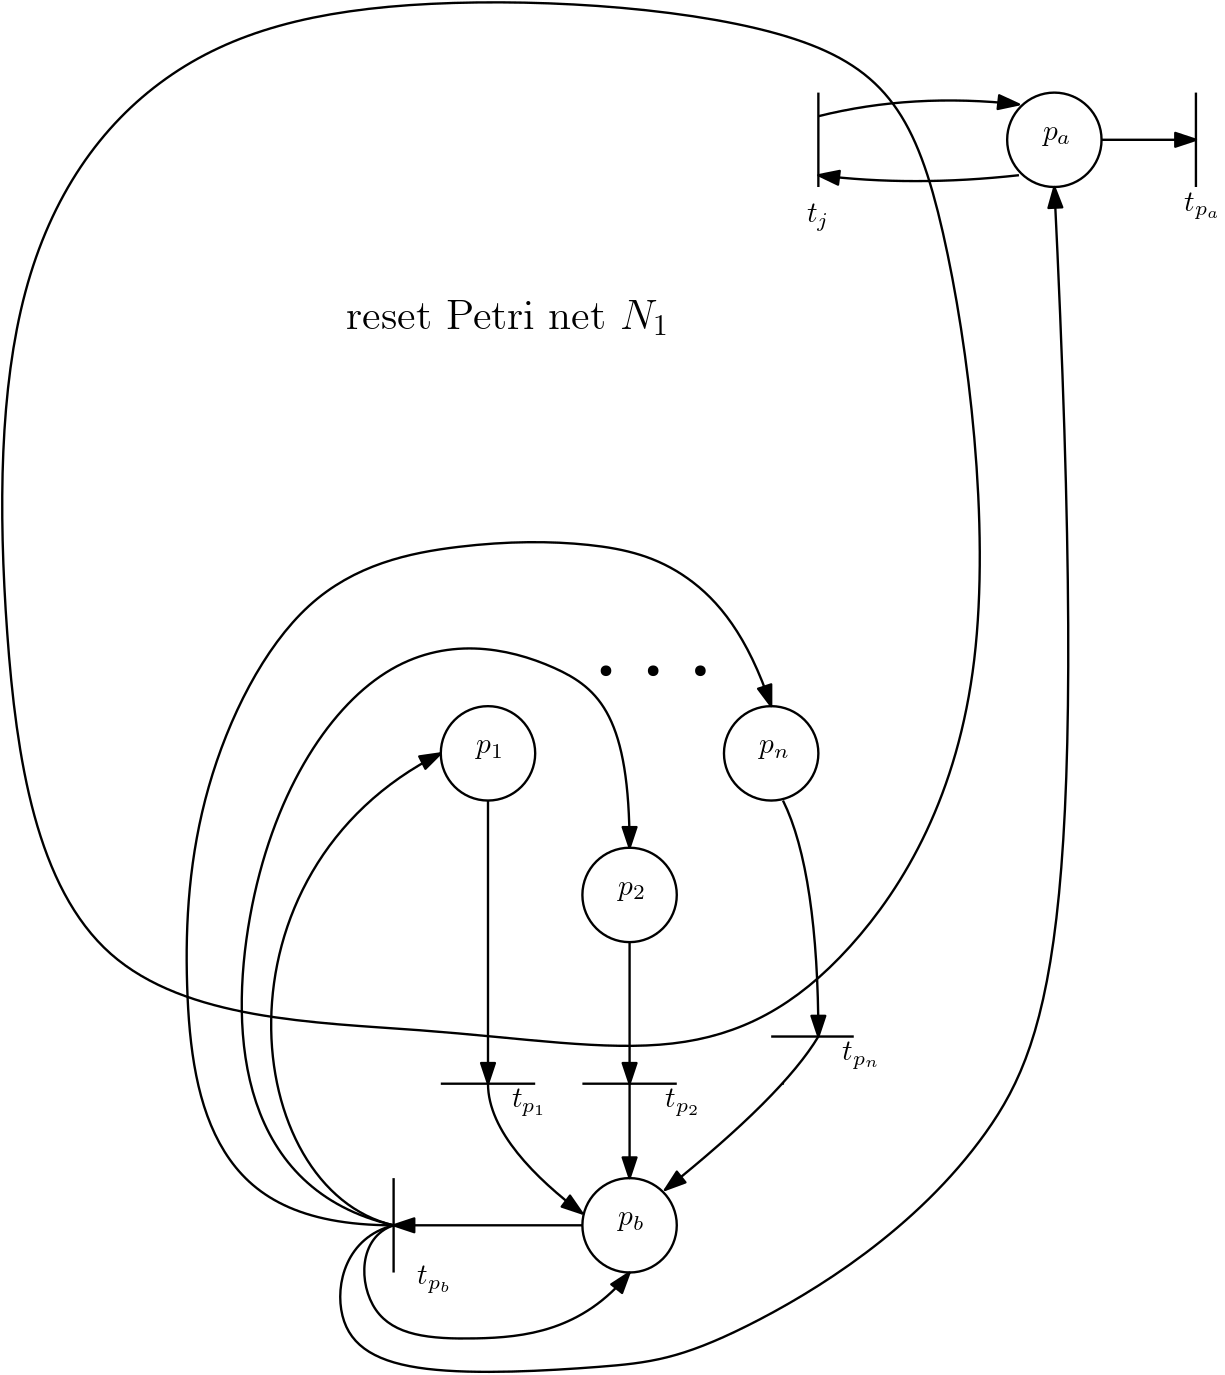
\includegraphics[width=0.75\textwidth]{FigurePN}
\caption{Construction of $N_2$ from $N_1$.}
	\end{figure}
\end{center}

Let us now prove that $t_{p_2}$ is live in $N_2$ if and only if 
the zero marking
is not reachable from $\mu_1$ in $N_1$. \\


{\bf Suppose that the zero marking is reachable from $\mu_1$ in $N_1$, then $t_{p_2}$ is not live in $N_2$}.

Indeed the marking with zero in every place of $P_1$ and in $p_b$ is reachable in $N_2$, by executing the same sequence of transition firings. Then $t_{p_a}$ can fire, leading to the marking which assigns zero to every place of $P_2$. From this marking the transitions $t_p$ are not live and neither are the transitions inherited from $N_1$ nor $t_{p_a}$, and, finally, nor is $t_{p_2}$. Thus $t_{p_2}$ is not live in $N_2$. \\


{\bf Suppose that $t_{p_2}$ is not live in $N_2$, then the zero marking is reachable from $\mu_1$ in $N_1$}

Indeed, if $t_{p_2}$ is not live in $N_2$, then a marking $\mu$ must be reachable in which $\mu(p_2) = 0$ and there is no reachable state in which $p_2$ has a token (in particular, since we do not allow token removal from $p_2$, the marking $\mu$ must be reached in a sequence of transitions that do not place any token in $p_2$).
This means that no transition $t_p$ is live in $N_2$ in $\mu$ since any transition $t_p$ can place a token in $p_2$. 
Thus, every place of $P_2$ inherited from $N_1$ must be devoid of token. Moreover, since the marking $\mu$ must be reached  in a sequence of transitions that do not place any token in $p_2$, 
it can be reached without using the transitions $t_p$ or $t_{p_2}$. Since $t_{p_a}$ do not modify the places inherited from $P_1$ nor does it enable new transitions, the reachability of $\mu$ implies the reachability of a marking where every place of $P_2$ inherited from $P_1$ is devoid of token using only the transitions inherited from $N_1$. Thus the zero marking is reachable from $\mu_1$ in $N_1$.
\end{proof}











\end{document}
